\newif\ifstocanon
\stocanonfalse
\documentclass[11pt]{article}

\usepackage[utf8]{inputenc}
\usepackage[T1]{fontenc}
\usepackage{lmodern}
\usepackage[protrusion=true,expansion=true]{microtype}
\usepackage[margin=1in]{geometry}
\usepackage{amsmath,amssymb,amsthm,mathtools}
\usepackage{booktabs,array,tabularx,multirow}
\usepackage{enumitem}
\usepackage{float,caption}
\usepackage[dvipsnames,table]{xcolor}
\usepackage{fancyhdr}
\usepackage{listings}
\usepackage{tikz}
\usetikzlibrary{arrows.meta,positioning,calc,decorations.pathreplacing}

\definecolor{mahogany}{rgb}{0.70, 0.20, 0.05}
\definecolor{darkblue}{rgb}{0.05, 0.20, 0.60}
\definecolor{commentpurple}{rgb}{0.48, 0.14, 0.52}

\usepackage[colorlinks=true,linkcolor=darkblue,citecolor=mahogany,urlcolor=darkblue]{hyperref}
\usepackage[capitalize,nameinlink]{cleveref}

\allowdisplaybreaks
\emergencystretch=2.5em
\renewcommand{\topfraction}{0.92}
\renewcommand{\bottomfraction}{0.88}
\renewcommand{\textfraction}{0.07}
\renewcommand{\floatpagefraction}{0.80}

% Clean STOC page numbering style (matching Woodruff STOC/FOCS papers)
\fancypagestyle{pg}{
  \fancyhf{}
  \cfoot{--\ \thepage\ --}
  \renewcommand{\headrulewidth}{0pt}
}

% Lean 4 listing style and Unicode support for the short formal specification in Section 8
\DeclareUnicodeCharacter{2203}{\ensuremath{\exists}}
\DeclareUnicodeCharacter{2200}{\ensuremath{\forall}}
\DeclareUnicodeCharacter{2115}{\ensuremath{\mathbb{N}}}
\DeclareUnicodeCharacter{00D7}{\ensuremath{\times}}
\DeclareUnicodeCharacter{0393}{\ensuremath{\Gamma}}
\DeclareUnicodeCharacter{2227}{\ensuremath{\wedge}}
\DeclareUnicodeCharacter{2080}{\ensuremath{{}_0}}
\DeclareUnicodeCharacter{2265}{\ensuremath{\ge}}
\DeclareUnicodeCharacter{2264}{\ensuremath{\le}}

\lstdefinelanguage{Lean4}{
  morekeywords={theorem,def,inductive,where,deriving,fun,namespace,open,import},
  sensitive=true,
  morecomment=[l]{--},
  morestring=[b]",
}
\lstdefinestyle{leanstyle}{
  language=Lean4,
  basicstyle=\ttfamily\small,
  keywordstyle=\ttfamily\small\bfseries,
  commentstyle=\ttfamily\small\itshape\color{gray!70!black},
  frame=single,
  framesep=5pt,
  rulecolor=\color{black!40},
  columns=fullflexible,
  keepspaces=true,
  upquote=true,
  aboveskip=6pt,
  belowskip=6pt,
  extendedchars=true,
  literate=
    {∃}{{$\exists$}}1
    {∀}{{$\forall$}}1
    {ℕ}{{$\mathbb{N}$}}1
    {×}{{$\times$}}1
    {Γ}{{$\Gamma$}}1
    {∧}{{$\wedge$}}1
    {₀}{{${}_0$}}1
    {≥}{{$\ge$}}1
    {≤}{{$\le$}}1
}

% Theorem environments (unified per-section counter, Woodruff STOC style)
\newtheorem{theorem}{Theorem}[section]
\newtheorem{lemma}[theorem]{Lemma}
\newtheorem{proposition}[theorem]{Proposition}
\newtheorem{corollary}[theorem]{Corollary}
\newtheorem{claim}[theorem]{Claim}
\newtheorem{observation}[theorem]{Observation}
\newtheorem{fact}[theorem]{Fact}
\newcommand{\innercustomthm}{}
\newtheorem*{theorem*}{Theorem~\innercustomthm}
\newtheorem*{lemma*}{Lemma~\innercustomthm}
\newtheorem*{corollary*}{Corollary~\innercustomthm}
\theoremstyle{definition}
\newtheorem{definition}[theorem]{Definition}
\newtheorem{remark}[theorem]{Remark}

\crefname{theorem}{Theorem}{Theorems}
\Crefname{theorem}{Theorem}{Theorems}
\crefname{lemma}{Lemma}{Lemmas}
\Crefname{lemma}{Lemma}{Lemmas}
\crefname{proposition}{Proposition}{Propositions}
\Crefname{proposition}{Proposition}{Propositions}
\crefname{corollary}{Corollary}{Corollaries}
\Crefname{corollary}{Corollary}{Corollaries}
\crefname{claim}{Claim}{Claims}
\Crefname{claim}{Claim}{Claims}
\crefname{fact}{Fact}{Facts}
\Crefname{fact}{Fact}{Facts}
\crefname{definition}{Definition}{Definitions}
\Crefname{definition}{Definition}{Definitions}
\crefname{remark}{Remark}{Remarks}
\Crefname{remark}{Remark}{Remarks}
\crefname{section}{Section}{Sections}
\Crefname{section}{Section}{Sections}
\crefname{appendix}{Appendix}{Appendices}
\Crefname{appendix}{Appendix}{Appendices}
\crefname{table}{Table}{Tables}
\Crefname{table}{Table}{Tables}
\crefname{figure}{Figure}{Figures}
\Crefname{figure}{Figure}{Figures}

% Algorithm float and line-numbered step list
\floatstyle{ruled}
\newfloat{algorithm}{tbp}{loa}
\floatname{algorithm}{Algorithm}
\crefname{algorithm}{Algorithm}{Algorithms}
\Crefname{algorithm}{Algorithm}{Algorithms}

\newlist{algsteps}{enumerate}{3}
\setlist[algsteps]{label=\arabic*:, ref=\arabic*, leftmargin=2.2em, itemsep=2.5pt, topsep=4pt, parsep=0pt, before=\raggedright}
\crefname{algstepsi}{Line}{Lines}
\Crefname{algstepsi}{Line}{Lines}

\newcommand{\algcomment}[1]{\hfill $\triangleright$~{\small\color{commentpurple} #1}}

% Self-contained restatable theorem/lemma/corollary support
\makeatletter
\newcounter{restate@savedeq}
\NewDocumentEnvironment{restatable}{O{} m m +b}{%
  \expandafter\xdef\csname #3@eq\endcsname{\the\c@equation}%
  \expandafter\gdef\csname #3\endcsname{%
    \begingroup
    \setcounter{restate@savedeq}{\value{equation}}%
    \setcounter{equation}{\csname #3@eq\endcsname}%
    \renewcommand{\theHequation}{restate.#3.\theequation}%
    \renewcommand{\label}[1]{}%
    \let\ltx@label\@gobble
    \let\label@in@display\@gobble
    \ifx&#1&%
      \begin{#2*}#4\end{#2*}%
    \else%
      \begin{#2*}[#1]#4\end{#2*}%
    \fi%
    \setcounter{equation}{\value{restate@savedeq}}%
    \endgroup
  }%
  \ifx&#1&%
    \begin{#2}#4\end{#2}%
  \else%
    \begin{#2}[#1]#4\end{#2}%
  \fi%
}{}
\newcommand{\restatethm}[2]{%
  \begingroup
  \renewcommand{\innercustomthm}{\ref{#2}}%
  \csname #1\endcsname
  \endgroup
}
\makeatother

% Mathematical macros
\newcommand{\C}{\mathbb{C}}
\newcommand{\R}{\mathbb{R}}
\newcommand{\Z}{\mathbb{Z}}
\newcommand{\Q}{\mathbb{Q}}
\newcommand{\N}{\mathbb{N}}
\newcommand{\F}{\mathbb{F}}
\newcommand{\Cg}{\widetilde{\mathbb{C}}}
\newcommand{\Rg}{\widetilde{\mathbb{R}}}
\newcommand{\Disk}{\mathbb{D}}
\newcommand{\Rr}{\mathcal{R}}
\newcommand{\cA}{\mathcal{A}}
\newcommand{\cF}{\mathcal{F}}
\newcommand{\Quant}{\mathcal{Q}}
\newcommand{\sinc}{\operatorname{sinc}}
\newcommand{\erf}{\operatorname{erf}}
\newcommand{\erfc}{\operatorname{erfc}}
\newcommand{\diag}{\operatorname{diag}}
\newcommand{\rank}{\operatorname{rank}}
\newcommand{\wt}{\operatorname{wt}}
\newcommand{\CNOT}{\mathrm{CNOT}}
\newcommand{\CZ}{\mathrm{CZ}}
\newcommand{\eps}{\varepsilon}
\newcommand{\poly}{\operatorname{poly}}
\newcommand{\norm}[1]{\left\lVert #1 \right\rVert}
\newcommand{\abs}[1]{\left\lvert #1 \right\rvert}
\newcommand{\ip}[2]{\left\langle #1, #2 \right\rangle}

% Procedure macros
\newcommand{\Pack}{\textnormal{\textsc{Pack}}}
\newcommand{\Bridge}{\textnormal{\textsc{Bridge}}}
\newcommand{\Spread}{\textnormal{\textsc{Spread}}}
\newcommand{\TensorFFT}{\textnormal{\textsc{TensorFFT}}}
\newcommand{\Deconvolve}{\textnormal{\textsc{Deconvolve}}}
\newcommand{\Recover}{\textnormal{\textsc{Recover}}}
\newcommand{\PositionalPerm}{\textnormal{\textsc{PositionalPerm}}}
% Additional convenience macros for compatibility
\providecommand{\SWAP}{\mathrm{SWAP}}
\providecommand{\DFT}{\mathrm{DFT}}
\providecommand{\IDFT}{\mathrm{IDFT}}
\providecommand{\cB}{\mathcal{B}}
\providecommand{\cO}{\mathcal{O}}
\providecommand{\cT}{\mathcal{T}}
\providecommand{\Emid}{\mathcal{E}_{\mathrm{mid}}}

\begin{document}

% ===== PART 1 =====
\title{A Simpler Algorithm for Integer Multiplication Below
\texorpdfstring{$n \log n$}{n log n},\\ with a Formally Verified Proof}
\ifcsname ifstocanon\endcsname\else
\expandafter\newif\csname ifstocanon\endcsname
\fi
\ifstocanon\author{Anonymous Author(s)}\else
\author{
Piaoyang Cui \\ {\small Google DeepMind} \and
Yiming Liu \\ {\small Google DeepMind} \and
David P.~Woodruff \\ {\small Google Research \& Carnegie Mellon University}
}
\fi
\date{}
\hypersetup{pageanchor=false}
\setcounter{page}{0}
\maketitle
\thispagestyle{empty}

\begin{abstract}
Sch\"onhage and Strassen conjectured that multiplying two $n$-bit integers requires $\Omega(n\log n)$ time on multitape Turing machines. Harvey and van der Hoeven attained $O(n\log n)$, and a recent OpenAI preprint obtained $O\bigl(n(\log n)^{1-\kappa}\bigr)$ time using two fixed finite linear networks. We give a simpler construction around those networks, together with a machine-checked proof.

Short convolutions replace cross-axis Fourier phases by fractional shifts on one power-of-two grid. A small complex phase separates two frequency contributions that would otherwise tie, allowing stable recovery of the original transform. The FFT's own pairwise sums and differences also permute address-bit positions exactly, eliminating separate data-reordering passes. These changes allow a direct complex tensor FFT without Chinese remainder theorem (CRT) reductions, grid expansion, Bluestein transforms, or a polynomial-ring middle transform.

The written proof gives $\kappa=2^{-56}$ at the preprint's unchanged tape-primitive constants, where it obtains $2^{-182}$. An independent Lean~4 formalization proves the entire construction, including the networks and an inner multiplier, and gives $\kappa=2^{-46}$ using only Lean's three standard logical axioms. Both proofs count tape movement and rounding error. The networks become useful only at astronomical input sizes, and we claim no practical speedup.
\end{abstract}

\clearpage
\hypersetup{pageanchor=true}
\pagestyle{pg}
\setcounter{page}{1}

\section{Introduction}\label{sec:intro}
\subsection{Integer Multiplication on Sequential Tapes}\label{sec:history}

How many steps are needed to multiply two $n$-bit integers?
We use deterministic multitape Turing machines, with a fixed finite alphabet, fixed control, and a fixed number of one-dimensional tapes.
Every tape-head movement counts.

A Fourier reduction splits the inputs into $\Theta(\log n)$-bit digits and computes a convolution of length $R=\Theta(n/\log n)$.
Recovering sums of up to $R$ digit products requires precision $P=\Theta(\log n)$, so the data occupy volume $V=\Theta(RP)=\Theta(n)$ bits.
Although an FFT uses only $O(R\log R)=O(n)$ arithmetic operations, a tape head cannot jump to a distant entry.
Scanning or rearranging this volume at each of the $\Theta(\log n)$ FFT stages costs $\Theta(n\log n)$ head steps, even if arithmetic is free.
This is a limitation of that implementation strategy, not a general lower bound.

Sch\"onhage and Strassen~\cite{SS71} achieved $O(n\log n\log\log n)$ time in 1971 and conjectured an $\Omega(n\log n)$ lower bound.
Later work reduced the overhead~\cite{Fur07,Fur09,DKSS13,HvdHL16}, until Harvey and van der Hoeven~\cite{HvdH21} reached $O(n\log n)$.
The recent integer-multiplication and exact-DFT preprints~\cite{OAI26,OAI26b} obtain a power saving below $n\log n$; see \Cref{tab:intmul-history}.

\begin{table}[htbp]
\centering\footnotesize
\setlength{\tabcolsep}{4pt}
\renewcommand{\arraystretch}{1.05}
\begin{tabularx}{\linewidth}{@{}>{\raggedright\arraybackslash}X
>{\raggedright\arraybackslash}p{0.27\linewidth}
>{\raggedright\arraybackslash}X@{}}
\toprule
\textbf{Reference} & \textbf{Running time} & \textbf{Main technique}\\
\midrule
Sch\"onhage--Strassen~\cite{SS71}
& $O(n\log n\log\log n)$ & Recursive Fermat-ring FFTs\\
F\"urer~\cite{Fur07,Fur09}; De et al.~\cite{DKSS13}
& $n\log n\,2^{O(\log^* n)}$ & Synthetic roots in polynomial rings\\
Harvey--van der Hoeven--Lecerf~\cite{HvdHL16}
& $O(n\log n\,8^{\log^* n})$ & Sharpened synthetic-root construction\\
Harvey--van der Hoeven~\cite{HvdH21}
& $O(n\log n)$ & Multi-prime CRT and Gaussian resampling\\
OpenAI~\cite{OAI26}
& $O\bigl(n(\log n)^{1-\kappa}\bigr)$ & Fixed networks; multi-grid Bluestein construction\\
This paper
& $O\bigl(n(\log n)^{1-\kappa}\bigr)$ & Fixed networks on one power-of-two grid\\
\bottomrule
\end{tabularx}
\caption{Deterministic multitape multiplication. Here $\kappa>0$ is an explicit constant, and $\log^* n$ is the iterated logarithm.}
\label{tab:intmul-history}
\end{table}

The saving in~\cite{OAI26} comes from two fixed finite linear networks that batch exchanges of address fields (blocks of address bits) and Fourier butterflies (pairwise sums and differences).
We ask whether these networks can support multiplication on one power-of-two grid, with a complete machine-checked proof.

\subsection{Our Results}\label{sec:results}

We keep one grid by representing fractional shifts with short convolutions and permuting address-bit positions by exact butterfly cancellations.
This gives a direct complex tensor FFT, which applies a Fourier transform along each axis.
The written proof imports exactly the tape primitives of \cite[Lemmas~3--4, Lemma~12, and Proposition~14]{OAI26} at their printed constants (\Cref{fact:streams,fact:interchange,fact:butterfly}).
We prove the remaining analytic and algorithmic steps, including precision and tape-layout bounds.

\begin{restatable}[Single-grid integer multiplication]{theorem}{thmmain}\label{thm:main}
There is a deterministic multitape Turing machine with a fixed finite alphabet and a fixed finite number of tapes that multiplies two $n$-bit integers in worst-case time
\[
 O\bigl(n(\log n)^{1-\kappa}\bigr),\qquad \kappa=2^{-56}.
\]
The machine in \Cref{alg:main} uses one grid $R=t_1\cdots t_d=2^k$, fractional-shift kernels with two-term cyclic solvers, and a direct complex tensor FFT.
Above a fixed cutoff $n_*$, all delegated integer products have $O((\log n)^2)$-bit operands.
These products and inputs below $n_*$ use any fixed independent deterministic multiplier of cost $\mathsf{M}(N)=N(\log N)^{O(1)}$, such as~\cite{SS71}; there is no self-recursion.
\end{restatable}

\begin{theorem}[Formally verified bound]\label{thm:lean}
The Lean~4 formalization~\cite{dMU21,mC20,Lean26} proves the entire construction from scratch in Mathlib's finite-alphabet multi-stack Turing machine model over $\N$, certifying worst-case time $O\bigl(n(\log n)^{1-\kappa}\bigr)$ with $\kappa=2^{-46}$.
It proves both $h=100$ networks, all stream, field-interchange, and butterfly primitives, and the sharpened leaf-cutoff and guard bounds
\[
 (\beta,C_1,1-\tau,1-\sigma)=(1/64,14,2^{-40},2^{-42}).
\]
Here $\beta$ controls when network recursion stops, $C_1$ is the degree of the temporary-precision bound, and $\tau,\sigma$ are the interchange and butterfly exponents.
It also proves an independent two-dimensional $O(N\log N)$ inner multiplier~\cite{MS}.
The proof uses only Lean's three standard logical axioms, \texttt{propext}, \texttt{Classical.\allowbreak choice}, and \texttt{Quot.\allowbreak sound}.
It assumes no result from~\cite{OAI26,HvdH21}.
\end{theorem}

\paragraph{How to read the results.}
\Cref{sec:multiplier} proves the written bound, charging every tape movement and rounding error.
Its recursive tape routines and independent short products never invoke the new multiplier itself.
The \href{https://github.com/lockqueue/intmul}{Lean proof} also checks the primitives; raising its time bound to the power $2^{46}$ allows a specification in natural-number arithmetic.
\Cref{sec:lean} explains the finite-alphabet clause (no unbounded integers in one cell), the tape simulation, and the trusted kernel and axioms.
The full paper~\cite{Full26} gives the complete analysis in greater detail; the companion paper~\cite{MS} develops the independent two-dimensional $O(N\log N)$ multiplier that serves as the inner multiplier in the formalization.

Both bounds are galactic: the fixed $h=100$, $m=10^6$ networks become useful only at astronomical input sizes.
Our exact-arithmetic Python package~\cite{Code26} tests the multi-axis pipeline with small substitute networks and checks the $h=100$ certificates symbolically, rather than executing those networks at their required sizes.
We claim neither a practical speedup nor a practical implementation of the large-network algorithm.

\begingroup
\setlength{\textfloatsep}{10pt plus 2pt minus 2pt}
\setlength{\intextsep}{7pt plus 2pt minus 2pt}
\captionsetup[figure]{skip=6pt}
\captionsetup[table]{skip=6pt}
\section{Overview}\label{sec:overview}

\subsection{What the Fixed Networks Provide}

Strassen's $2\times2$ identity replaces eight block multiplications by seven and linear combinations.
Repeating it changes the exponent from $3$ to $\log_2 7$.
The tape networks use the same principle: a fixed reduction in the number of smaller calls changes an exponent.

A \emph{role} is one of $W$ equal-length data streams on separate tapes.
A width-$m$ task groups $m$ elementary operations per role, while a width-$1$ call performs one elementary operation.
The direct implementation therefore takes $Wm$ calls, whereas a network uses $s<Wm$ calls and $O(V)$ linear-combination work on $V$ data bits.
Dividing by the number of roles gives the \emph{normalized count} $s/W$.
If $s/W<m^\gamma$ for some $\gamma<1$, then $t$ levels handle width $u=m^t$ with normalized count
\[
 (s/W)^t\le (m^t)^\gamma=u^\gamma,
\]
rather than $u$; the constants $W,m,s$ remain fixed.

The two identities of~\cite{OAI26}, with $h=100$ and $m=h^3=10^6$, give exponents $\tau,\sigma<1$ for field interchange and butterfly recursion, respectively.
The printed interchange routine exchanges two disjoint $u$-bit address fields in $O(V(1+u^\tau))$ time; the butterfly routine accepts the following layout.

We store the length-$R$ vector on one tape as a balanced $d$-axis array: for fixed $\eps,c>0$, choose
\[
 R=2^k=t_1\cdots t_d,\qquad
 d=\lfloor k^\eps\rfloor,\quad \ell=\lceil k/d\rceil,\quad
 t_d=r=2^\ell,\quad t_a\in\{r/2,r\}.
\]
We work above a fixed cutoff with $d\ge2$.
Axis $d$ varies fastest, so its $r$ contiguous complex entries form one \emph{record}, and there are $M=R/r=2^{m_0}$ records.
An $m_0$-bit counter supplies the record address, which is not stored with the data.
At working precision $P$, we use $q=P+2$ fractional bits and width $w=q+2$ per real or imaginary component, giving volume $V=2Mrw=\Theta(RP)$.

A \emph{chunk} consists of $K=\lfloor d^c\rfloor$ consecutive record-address bits.
A \emph{slice} selects the same offset in each of $D\le d$ consecutive chunks.
For illustration, offset $1$ from the least significant end of
$(x_5x_4x_3\mid x_2x_1x_0)$ selects $x_4,x_1$.

A butterfly on one address bit pairs records differing only at that bit and applies
$H_0(u,v)=((u+v)/2,(u-v)/2)$ to corresponding entries.
One parallel call applies the tensor product of these maps on the entire slice, rounding only its final output.
It cannot skip individual slice bits: the interface specifies whole chunks and a common offset, not an arbitrary subset.
Its cost is $O(Vd^{\lambda'})$ for a fixed $\lambda'<1$, including the network's implementation on fixed tapes (\Cref{fact:butterfly}).

If the current bit of every outer axis occupies a slice, one call performs a Fourier round across those axes.
There are $\ell$ rounds, and our parameters give $V=\Theta(n)$ and $k=\Theta(\log n)$.
Since $\ell=\Theta(k/d)$, their cost is
\[
 O(V\ell d^{\lambda'})
 =O(Vk\,d^{\lambda'-1})
 =O\bigl(n(\log n)^{1-\eps(1-\lambda')}\bigr).
\]
We must connect multiplication to these rounds without spending $O(n\log n)$ elsewhere.

\subsection{The Multiplication Pipeline}

Let $\mathbf a,\mathbf b\in\R^R$ be digit vectors padded to at least twice their original length, so that cyclic convolution, denoted $\circledast$, equals ordinary convolution.
Packing them into $z=\mathbf a+i\mathbf b$ gives
\[
 z\circledast z
 =\mathbf a\circledast\mathbf a-\mathbf b\circledast\mathbf b
   +2i(\mathbf a\circledast\mathbf b),
\]
so its imaginary part isolates twice the desired product.

We use the normalized forward transform
$(\cF_Rw)_u=R^{-1}\sum_{j<R}w_j e^{2\pi iju/R}$.
Conjugation reverses the Fourier sign, giving
$\cF_R(\overline{\cF_Rw})=R^{-1}\overline w$.
The convolution theorem gives
$\cF_R(z\circledast z)=R(\cF_Rz)\odot(\cF_Rz)$, where $\odot$ is entrywise multiplication.
Thus a second forward call on the conjugated square returns $\overline{z\circledast z}/R^2$, and
\[
 \mathbf a\circledast\mathbf b
 =-\frac{R^2}{2}\operatorname{Im}
 \cF_R\!\left(\overline{(\cF_Rz)\odot(\cF_Rz)}\right).
\]
The conjugate lets us reuse the forward routine instead of building a separate inverse.

Each forward call is implemented by $\Bridge$, the three middle stages in \Cref{fig:pipeline}.
Spreading represents fractional sample positions on the integer grid, $\TensorFFT$ transforms along each axis, and deconvolution recovers the one-dimensional Fourier coefficients.
Write $\Cg_q=2^{-q}(\Z+i\Z)$ for the fixed-point grid and $\Quant_q$ for coordinatewise nearest rounding, with ties to even.
The precision in \Cref{alg:main} leaves coefficient error below $1/2$, so integer rounding and carry propagation recover the exact product (\Cref{prop:root-packing}).

\begin{figure}[htbp]
\centering
\resizebox{\linewidth}{!}{%
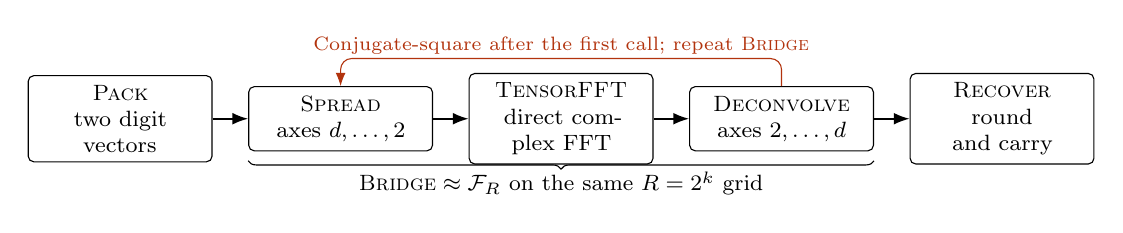
\begin{tikzpicture}[>=Latex,
s/.style={draw,rounded corners=2pt,text width=2.1cm,minimum height=.78cm,align=center,font=\footnotesize}]
\node[s] (p) at (0,0) {\textbf{\Pack}\\two digit vectors};
\node[s] (s) at (2.8,0) {\textbf{\Spread}\\axes $d,\ldots,2$};
\node[s] (f) at (5.6,0) {\textbf{\TensorFFT}\\direct complex FFT};
\node[s] (d) at (8.4,0) {\textbf{\Deconvolve}\\axes $2,\ldots,d$};
\node[s] (r) at (11.2,0) {\textbf{\Recover}\\round and carry};
\foreach \a/\b in {p/s,s/f,f/d,d/r} \draw[->,semithick] (\a.east)--(\b.west);
\draw[->,mahogany,rounded corners] (d.north)--++(0,.35)-|(s.north);
\node[font=\scriptsize,text=mahogany] at (5.6,.93) {Conjugate-square after the first call; repeat \Bridge};
\draw[decorate,decoration={brace,mirror,amplitude=3pt}]
($(s.south west)+(0,-.12)$)--($(d.south east)+(0,-.12)$);
\node[font=\footnotesize] at (5.6,-.82) {$\Bridge\approx\cF_R$ on the same $R=2^k$ grid};
\end{tikzpicture}}
\caption{The three middle boxes form one forward call. Follow the return arrow once, conjugate-squaring between calls; recovery follows the second call.}
\label{fig:pipeline}
\end{figure}

\begin{algorithm}[htbp]
\caption{Integer multiplication on one power-of-two grid}\label{alg:main}
\small
\setlist[algsteps]{label=\arabic*:, ref=\arabic*, leftmargin=2.2em, itemsep=1pt, topsep=2pt}
\textbf{Input:} $0\le A,B<2^n$. \textbf{Output:} $AB$.\\
\textbf{Parameters for $n\ge n_*$:}
$b=\lfloor\log_2n\rfloor$, $N_{\mathrm{dig}}=\lceil n/b\rceil$,
least power of two $R=2^k\ge2N_{\mathrm{dig}}$, and balanced axes.
Set $p=2b+2k+6$; use the precision schedule of \Cref{thm:bridge-acc} and the parameter choices of \Cref{lem:root-family}.
\begin{algsteps}
\item If $n<n_*$, return the product from the independent multiplier $\mathsf{M}$.
\item $x\leftarrow\Pack(A,B)$: set $x_j=2^{-b}(a_j+ib_j)$ from radix-$2^b$ digits, with zero padding.
\item $\hat y\leftarrow\Bridge(x)$.
\item $\hat w\leftarrow\Quant_{p+2}\bigl(\overline{\hat y\odot\hat y}\bigr)$.
\item $\hat z\leftarrow\Bridge(\hat w)$.
\item Return $\Recover(\hat z)$: round $-2^{2b-1}R^2\operatorname{Im}\hat z_j$ to integers and propagate carries.
\end{algsteps}
\smallskip\hrule\smallskip
\textbf{Subroutine $\Bridge(x)$.}
Use the power-of-two scale $S$ and fixed-point operations of \Cref{alg:bridge}.
The kernels $g_a$, offsets $\delta_a$, and mixing weights $c_0,c_1$ are described below; put $A_a=\prod_{i<a}t_i$.
\begin{algsteps}[resume]
\item Set $U\leftarrow x/S$ exactly and reverse the input axis fields to tensor order.
For $a=d,\ldots,2$, spread along axis $a$ using $g_a$ at offsets $\delta_a$.
\item $Y\leftarrow\TensorFFT(U)$.
\item For $a=2,\ldots,d$, solve
$c_0Z_f+c_1Z_{(f-R/A_a)\bmod R}=Y_f$ for $0\le f<R$ by the rounded two-pass cyclic solver; set $Y\leftarrow Z$.
\item Return $\Quant_{p+2}(SY)$.
\end{algsteps}
\end{algorithm}

\paragraph{Two obstacles.}
A tensor DFT omits the cross-axis phases of the one-dimensional DFT.
The CRT construction of~\cite{HvdH21,OAI26} separates the transform using coprime odd-prime axis lengths, and Gaussian resampling then interpolates onto larger power-of-two grids.
We instead account for the missing phases by fractional shifts on the existing grid.

The parallel primitive also requires aligned slices and supplies only the real butterfly $H_0$.
In~\cite{OAI26}, physical chunk swaps move address blocks into place, and Bluestein's chirp identity~\cite{Blu70} replaces Fourier phases by convolution with quadratic-phase sequences.
Polynomial transforms~\cite{NQ78,Nus80} compute these convolutions over $\C[y]/(y^r+1)$, using coefficient shifts to implement roots of unity.
We instead use exact address-bit permutations and a direct complex tensor FFT (\Cref{tab:comparison}).

\begin{table}[htbp]
\centering\footnotesize
\setlength{\tabcolsep}{4pt}
\renewcommand{\arraystretch}{1.04}
\begin{tabularx}{\linewidth}{@{}>{\raggedright\arraybackslash}X
>{\raggedright\arraybackslash}X
>{\raggedright\arraybackslash}p{0.16\linewidth}@{}}
\toprule
\textbf{Prior construction~\cite{HvdH21,OAI26}}
& \textbf{Single-grid construction} & \textbf{Analysis}\\
\midrule
CRT and Gaussian grid expansion & Fractional shifts on the unchanged $2^k$ grid & \Cref{sec:bridge}\\
$O(d^2)$ adjacent axis swaps & $O(d)$ direct swaps with the innermost axis & \Cref{lem:axis-swap}\\
Physical width-$K$ chunk swaps & Bit-exact address permutations from butterflies & \Cref{thm:pos-perm}\\
Bluestein chirps and polynomial-ring convolutions & Direct complex tensor FFT & \Cref{thm:direct-fft}\\
Middle error amplified by $M$; output widening & Error $<12\ell\,2^{-q}$; no output widening & \Cref{cor:walsh-middle}\\
$\Theta(rP)$-bit packed polynomial products & $O(P^2)$-bit delegated products & \Cref{sec:mult-cost}\\
\bottomrule
\end{tabularx}
\caption{Changes around the shared networks. Axis swaps remain in spreading; separate chunk-swap layout passes inside the middle transform are removed.}
\label{tab:comparison}
\end{table}

\subsection{Idea 1: Fractional Shifts on One Grid}

The missing cross-axis phases can be represented as fractional sample positions.
For two axes, write $R=t_1r$, input position $j=j_1+t_1j_2$, and output frequency $f=u_1r+u_2$.
These use opposite axis orders; the initial field reversal in \Cref{alg:main} converts the input to tensor order.
Expanding the Fourier phase gives
\[
 \frac{jf}{R}
 =\frac{j_1u_1}{t_1}
  +\left(j_2+\frac{j_1}{t_1}\right)\frac{u_2}{r}+j_2u_1.
\]
The integer term $j_2u_1$ disappears from the exponential, leaving axis-$2$ samples at positions $j_2+\delta$, where $\delta=j_1/t_1$.
For illustration, with $t_1=2,r=4$, even-indexed input samples lie at integer positions and odd-indexed samples at half-integer positions.
We must represent this half-cell displacement on the integer grid.

We do so by a short convolution.
The ideal interpolation kernel $\sinc(s)=\sin(\pi s)/(\pi s)$, with $\sinc(0)=1$, decays too slowly, so we damp it by a Gaussian:
\[
 g_0(s)=\sinc(s)e^{-\pi s^2/\alpha^2},
 \qquad
 G(\xi)=\int_{\xi-1/2}^{\xi+1/2}\alpha e^{-\pi\alpha^2v^2}\,dv.
\]
Here $G$ is the Fourier transform of $g_0$ (with kernel $e^{-2\pi i\xi s}$), and \Cref{def:carrier} chooses the width $\alpha$ from a parameter $\omega$ that controls the exponentially small tails.
For a kernel $g$, a sample at $j_2+\delta$ contributes $g(j_2-h+\delta)$ at integer position $h$.
We retain only the $2P+1$ integer offsets $-P,\ldots,P$, called \emph{taps}, and then fold indices modulo $r$; no grid points are added (\Cref{lem:bridge-fp,thm:bridge-acc}).

Sampling a kernel on integers creates shifted frequency copies, called \emph{aliases}.
Before truncation and scaling, Poisson summation gives
\[
 (\cF_{t_1,r}U)_{u_1,u_2}
 =\sum_{\nu\in\Z}\widehat g\left(\frac{u_2}{r}-\nu\right)
   (\cF_Rx)_{((u_1-\nu)\bmod t_1)r+u_2}.
\]
For fixed $u_2$, write $Y_{u_1}$ for this output and $Z_{u_1}=(\cF_Rx)_{u_1r+u_2}$.
With $g=g_0$, the weights $c_0=G(u_2/r)$ and $c_1=G(u_2/r-1)$ dominate: all other aliases have total weight $O(2^{-\omega})$.
Recovery therefore requires undoing the cyclic mixture
$Y_{u_1}\approx c_0Z_{u_1}+c_1Z_{(u_1-1)\bmod t_1}$.

\paragraph{Separating the two aliases.}
The real kernel fails at the midpoint frequency, called the Nyquist bin.
At $u_2=r/2$, evenness gives $c_0=G(1/2)=G(-1/2)=c_1$.
The retained mixing map $c_0(I+T)$, where $T$ shifts once around the cycle, annihilates $(1,-1,1,-1,\ldots)$ on even cycles.

Every real kernel has the same magnitude obstruction: Hermitian symmetry,
$\widehat g(-\xi)=\overline{\widehat g(\xi)}$, ties the alias magnitudes at $1/2$.
If $c_1\ne0$, some $L$th root of unity $\zeta$ lies within $\pi/L$ of $-c_0/c_1$, so $|c_0+c_1\zeta|\le\pi|c_1|/L$.
Its Fourier eigenvector forces inverse norm at least $L/(\pi|c_1|)$ whenever the inverse exists.
Since the cycle at axis $a$ has length $A_a=\prod_{i<a}t_i$, paying this factor at every axis (for bounded weights) costs
$\sum_{a=2}^d\log_2 A_a=\Theta(dk)$ bits on a balanced grid, instead of $O(k)$.

We break the symmetry by multiplying the kernel by a small complex phase, called a \emph{carrier}.
The negative half-bin sign gives
\[
 g_a(s)=e^{-\pi is/t_a}g_0(s),\qquad
 \widehat g_a(\xi)=G\left(\xi+\frac1{2t_a}\right),\qquad
 y=\frac{u_a+1/2}{t_a}.
\]
Now $c_0=G(y)$ and $c_1=G(y-1)$.
Since $t_a$ is even, every sampled $y$ lies inside $(0,1)$ and at distance at least $1/(2t_a)$ from $1/2$ (\Cref{fig:nyquist}).
For $B_a=c_0I+c_1T$, \Cref{lem:bridge-cond} shows $|c_0-c_1|\ge\frac7{4t_a}$, so the amplification of maximum-entry error is $\norm{B_a^{-1}}_\infty\le1/|c_0-c_1|\le\frac47t_a$, independently of the cycle length.

\begin{figure}[htbp]
\centering
\resizebox{.95\linewidth}{!}{%
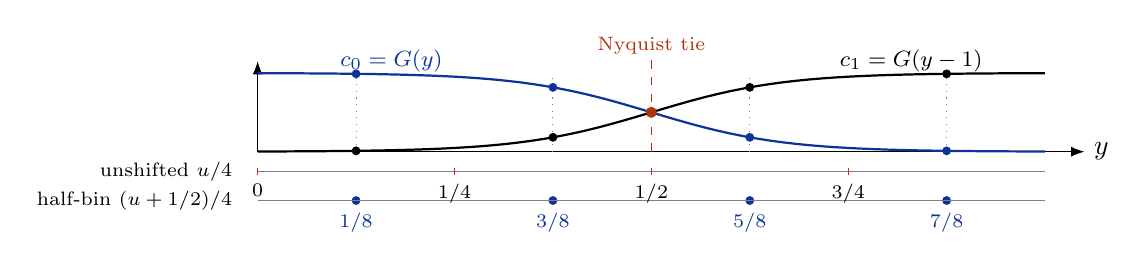
\begin{tikzpicture}[>=Latex,x=10cm,y=1cm]
\draw[->] (0,0)--(1.05,0) node[right] {$y$};
\draw[->] (0,0)--(0,1.15);
\draw[thick,darkblue,domain=0:1,samples=61] plot (\x,{1/(1+exp(12*(\x-.5)))});
\draw[thick,domain=0:1,samples=61] plot (\x,{1/(1+exp(-12*(\x-.5)))});
\node[font=\footnotesize,text=darkblue] at (.17,1.15) {$c_0=G(y)$};
\node[font=\footnotesize] at (.83,1.15) {$c_1=G(y-1)$};
\draw[dashed,mahogany] (.5,0)--(.5,1.17);
\node[font=\scriptsize,text=mahogany] at (.5,1.35) {Nyquist tie};
\fill[mahogany] (.5,.5) circle (2pt);
\foreach \x in {.125,.375,.625,.875} {
\draw[dotted,gray] (\x,0)--(\x,1);
\fill[darkblue] (\x,{1/(1+exp(12*(\x-.5)))}) circle (1.6pt);
\fill (\x,{1/(1+exp(-12*(\x-.5)))}) circle (1.6pt);
\fill[darkblue] (\x,-.62) circle (1.6pt);}
\draw[gray] (0,-.25)--(1,-.25);
\draw[gray] (0,-.62)--(1,-.62);
\node[anchor=east,font=\scriptsize] at (-.02,-.25) {unshifted $u/4$};
\node[anchor=east,font=\scriptsize] at (-.02,-.62) {half-bin $(u+1/2)/4$};
\foreach \x/\v in {0/0,.25/{1/4},.5/{1/2},.75/{3/4}} {
\draw[mahogany] (\x,-.21)--(\x,-.29);
\node[font=\scriptsize,anchor=north] at (\x,-.29) {$\v$};}
\foreach \x/\v in {.125/{1/8},.375/{3/8},.625/{5/8},.875/{7/8}}
\node[font=\scriptsize,anchor=north,text=darkblue] at (\x,-.66) {$\v$};
\end{tikzpicture}}
\caption{Schematic alias weights for $t_a=4$. The half-bin samples avoid the equal-weight crossing and stay inside $(0,1)$, unlike the unshifted samples.}
\label{fig:nyquist}
\end{figure}

The sign also matters for the omitted aliases.
A positive carrier puts $u_a=0$ at $y=-1/(2t_a)$, outside $(0,1)$, where the discarded $\nu=-1$ alias need not satisfy the uniform $O(2^{-\omega})$ tail bound.
The negative sign protects both the weight gap and the two-alias approximation (\Cref{sec:bridge-cond}).

\paragraph{Axis order.}
For several axes, the fractional shift on axis $a$ depends only on earlier input digits:
\[
 A_a=\prod_{i<a}t_i,\qquad
 \delta_a(\mathbf j)=\frac{\sum_{i<a}j_iA_i}{A_a},\qquad
 f(\mathbf u)=\sum_{a=1}^d u_a\frac{R}{A_{a+1}}.
\]
We spread in descending order $d,\ldots,2$, so those earlier digits remain unchanged until axis $a$ reads them.
The initial field reversal makes axis $d$ contiguous, while tensor frequency order agrees with increasing $f$.

Let $\cA_a$ mix all aliases of axis $a$, and put $\mathbf t=(t_1,\ldots,t_d)$.
For the exact, unscaled spread array, \Cref{lem:bridge-exact} gives
$\cF_{\mathbf t}U=\cA_2\cA_3\cdots\cA_d(\cF_Rx)$, with the rightmost operator acting first.
Subtracting $R/A_a$ changes only earlier frequency digits, which makes this ordered factorization work.
We remove the retained two-term factors from the outside in, starting with $B_2$ and proceeding in ascending order; they need not commute.
Their inverse norms multiply to at most
$\prod_{a=2}^d(4t_a/7)=(4/7)^{d-1}R/t_1\le R/t_1$, so the total loss needs only $O(k)$ extra precision bits (\Cref{lem:bridge-cond}).

\paragraph{Two-pass cyclic solves.}
Divide by the larger weight and orient the cycle to obtain
$Z_j=\widetilde Y_j-\rho Z_{j-1\bmod L}$, where
$\rho=\min(c_0,c_1)/\max(c_0,c_1)<1$.
For illustration, on a length-$4$ cycle a pass starting from seed zero ends at
\[
 \widetilde Y_3-\rho\widetilde Y_2+\rho^2\widetilde Y_1-\rho^3\widetilde Y_0
 =(1-\rho^4)Z_3.
\]
Dividing by $1-\rho^4$ recovers $Z_3$, and a second pass from that seed recovers $Z_0,Z_1,Z_2$.

In general, $L=A_a$ is an even power of two, so a trip around the cycle multiplies the unknown seed by $(-\rho)^L=\rho^L$.
The zero-seed endpoint is therefore $(1-\rho^L)Z_{L-1}$, and the same two-pass procedure applies.
Per-step recurrence errors accumulate geometrically, with amplification
\[
 \frac{1+\rho+\cdots+\rho^{L-1}}{1-\rho^L}
 =\frac1{1-\rho}.
\]
Even when $\rho$ is close to one, this factor depends on the weight gap, not on $L$; \Cref{lem:bridge-fp} also accounts for stored-coefficient errors and the closing division.

The cyclic solves need no transpose: writing $f=j(R/L)+s$, for each fixed column $s$ the successive rows $j$ form one cycle.
A side tape holds one $O(P)$-bit state per column, and each row sweep advances all states in lockstep.
Each pass has $O(V)$ scan overhead (\Cref{lem:bridge-fp}).

Spreading does need each axis to be contiguous.
We swap it directly with the innermost axis and then restore it, using $O(d)$ field swaps rather than $O(d^2)$ adjacent swaps.
\Cref{lem:axis-swap,lem:bridge-fp} give the tape costs and implement each short convolution using $O(P^2)$-bit integer products.

\paragraph{Scaling and rounding.}
The butterfly primitive requires inputs in the closed unit disk.
For the exact folded kernel $H_\delta^{(a)}$ of \Cref{def:carrier}, Poisson summation expresses each unnormalized Fourier coefficient as phases with nonnegative weights $G(y-\nu)$.
These weights sum to one because their defining integration intervals tile $\R$.
Parseval and Cauchy--Schwarz then give
$\norm{H_\delta^{(a)}}_2\le1$ and
$\norm{H_\delta^{(a)}}_1\le\sqrt{t_a}$, so spreading amplifies the sup norm by at most $\sqrt{R/t_1}$.

We therefore divide the input by a power of two $S$ that exceeds $X\sqrt{R/t_1}$, where $X=\max(1,\norm{x}_\infty)$, by a fixed safety factor; \Cref{alg:bridge,thm:bridge-acc} choose $S$ so that the division is exact and every computed spread, including its rounding errors, stays in the disk.

Two rounding rules serve different purposes.
Coordinatewise truncation toward zero, $Q_q$, cannot increase either coordinate's magnitude, so butterflies, permutations, and disk products use it to preserve $\Disk_q=\{z\in\Cg_q:|z|\le1\}$.
Nearest rounding $\Quant_q$ halves the worst-case coordinate error but can leave the disk: at mesh $1/2$, $(3+4i)/5$ rounds to $1/2+i$.
We use nearest rounding in spreading and deconvolution, where separate modulus bounds allow this increase.

For $p\ge\max(8,k)$, working precision $P=O(p+k)$ suffices even as $d$ grows.
For $x\in\Cg_{p+2}^R$ with $\norm{x}_\infty\le2^p$, \Cref{thm:bridge-acc} gives maximum-entry error
$\norm{\Bridge(x)-\cF_Rx}_\infty<2^{-p}X/4$, including tap truncation, omitted aliases, cyclic solves, and rescaling.
That theorem specifies $\omega,P,q,w$ and all safety margins.
Taps, solver scalars, and phases use certified rational power-series approximations, not a transcendental rounding oracle (\Cref{lem:app-tables}).

\subsection{Idea 2: Exact Permutations of Address Bits}

The tensor FFT needs to rearrange record-address bits to align its parallel rounds.
We do this by temporarily mixing records and then canceling the mixing exactly.
For a two-bit illustration, a controlled flip sends
$(x_c,x_t)$ to $(x_c,x_t\oplus x_c)$, where $\oplus$ is addition modulo two.
It changes the target bit only when the control is one.
The identities
\[
 2H_0^2=I,\qquad
 2H_0\diag(1,-1)H_0=
 \begin{pmatrix}0&1\\1&0\end{pmatrix}
\]
give these two cases: two target-bit butterflies turn the recordwise sign $(-1)^{x_cx_t}$ into a controlled flip of the address.
The sign needs no routing, since an address counter determines whether to negate each record (\Cref{lem:long-scan}).

\paragraph{Selecting part of a slice.}
A parallel call acts on every bit of its slice, not just the desired targets.
We cancel its action on the other bits using $S_{\mathrm{ph}}=\diag(1,i)$ and the identities
\[
 H_0^3=\tfrac12H_0,\qquad
 (H_0S_{\mathrm{ph}})^3=\tfrac{1+i}{4}I.
\]
Let $T$ contain the $s$ selected bits and $U$ the other $D-s$ bits.
Before each of three full layers, apply the recordwise phase $i^{\sum_{u\in U}x_u}$.
Each selected bit leaves a factor $1/2$, and each unselected bit leaves the scalar $(1+i)/4$.
Multiplying afterward by $2^s[2(1-i)]^{D-s}$ therefore gives exactly $H_T$, the butterfly on $T$ alone.

For disjoint control-target pairs, the controlled sign
$(\CZ z)(x)=(-1)^{\sum_jx_{c_j}x_{t_j}}z(x)$ is also one scan.
A batch of controlled flips is
$\CNOT^{\otimes s}=2^sH_T\CZ H_T$, so it uses six full layers (\Cref{fig:walsh-circuits}).
Unselected bits are restored before $\CZ$ reads them, so they may serve as controls; controls may also lie far from the target slice.

\begin{figure}[htbp]
\centering
\resizebox{\linewidth}{!}{%
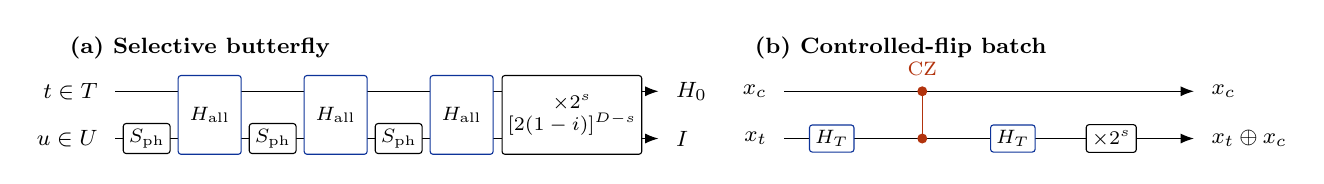
\begin{tikzpicture}[>=Latex,
g/.style={draw,fill=white,rounded corners=1pt,inner sep=2pt,font=\scriptsize},
h/.style={g,minimum height=10mm,minimum width=8mm}]
\node[anchor=west,font=\footnotesize\bfseries] at (0,.85) {(a) Selective butterfly};
\foreach \y/\v in {.3/{t\in T},-.3/{u\in U}} {
\draw[->] (.7,\y)--(7.6,\y);
\node[anchor=east,font=\footnotesize] at (.6,\y) {$\v$};}
\foreach \x in {1.1,2.7,4.3} \node[g] at (\x,-.3) {$S_{\mathrm{ph}}$};
\foreach \x in {1.9,3.5,5.1} \node[h,draw=darkblue] at (\x,0) {$H_{\mathrm{all}}$};
\node[h,align=center] at (6.5,0) {$\times 2^s$\\$[2(1-i)]^{D-s}$};
\node[font=\footnotesize,anchor=west] at (7.7,.3) {$H_0$};
\node[font=\footnotesize,anchor=west] at (7.7,-.3) {$I$};
\node[anchor=west,font=\footnotesize\bfseries] at (8.7,.85) {(b) Controlled-flip batch};
\foreach \y in {.3,-.3} \draw[->] (9.2,\y)--(14.4,\y);
\node[anchor=east,font=\footnotesize] at (9.1,.3) {$x_c$};
\node[anchor=east,font=\footnotesize] at (9.1,-.3) {$x_t$};
\foreach \x in {9.8,12.1} \node[g,draw=darkblue] at (\x,-.3) {$H_T$};
\draw[mahogany] (10.95,.3)--(10.95,-.3);
\foreach \y in {.3,-.3} \fill[mahogany] (10.95,\y) circle (1.8pt);
\node[font=\scriptsize,text=mahogany] at (10.95,.58) {$\CZ$};
\node[g] at (13.35,-.3) {$\times2^s$};
\node[anchor=west,font=\footnotesize] at (14.5,.3) {$x_c$};
\node[anchor=west,font=\footnotesize] at (14.5,-.3) {$x_t\oplus x_c$};
\end{tikzpicture}}
\caption{Classical linear circuits, read left to right. In (a), three full slice layers $H_{\mathrm{all}}$ cancel on $U$; in (b), two selective maps turn a controlled sign into controlled flips.}
\label{fig:walsh-circuits}
\end{figure}

Every permutation of address-bit positions factors into two involutions, each consisting of disjoint swaps and fixed positions.
This follows by expressing each cycle as two reflections (\Cref{lem:two-involutions}).
A swap uses three XOR updates:
$(a,b)\mapsto(a\oplus b,b)\mapsto(a\oplus b,a)\mapsto(b,a)$.
The two involutions therefore give six stages of disjoint controlled flips.
Grouping targets by slice, with leftover bits handled by elementary stream operations, gives total cost $O(V\ell d^{\lambda'})$ (\Cref{thm:pos-perm}).

\paragraph{Bit-exact implementation.}
Before each controlled-flip batch, append $8d$ zero fractional bits, giving precision $q_*=q+8d$.
Six layers on $D\le d$ bits divide by at most $2^{6D}$.
All phases and restoring scalars are Gaussian integers, with integer real and imaginary parts, so every exact layer-boundary value is representable on the lifted grid.
The imported primitive evaluates each layer without internal rounding and then applies $Q_{q_*}$ once; this truncation discards only zeros.

Every layer call also receives a disk-valued array: normalized layers and phases preserve the disk, and each restoring scalar is applied in steps that increase moduli only toward the completed value, which is a contraction or a permutation.
A completed batch merely permutes the original data, so removing the temporary bits is exact (\Cref{lem:lifting,prop:slice-cnot}).

We permute the $\Theta(\log n)$ address-bit positions, not arbitrary permutations of the $M$ records.
This includes a square power-of-two matrix transpose of these long records, since it exchanges two address fields.
The method uses long payloads and complex linear combinations that later cancel, so it gives no short-record routing bound in the transposition comparison of~\cite{HvdH25}.

\subsection{Idea 3: A Direct Tensor FFT}

Decimation in frequency (DIF) separates even and odd output frequencies.
On a length-$2h$ vector, one step forms $(z_j+z_{j+h})/2$ and $(z_j-z_{j+h})e^{2\pi ij/(2h)}/2$ for $0\le j<h$.
The first half feeds the even frequencies and the second feeds the odd frequencies of two length-$h$ transforms.
Recursing therefore extracts frequency bits in reverse order.

We first compute the length-$r$ FFT within each record, including local bit reversal.
For the outer axes, an exact layout $\mathcal L$ places the at most $(d-1)K$ bits that do not fill complete chunks at the front and interleaves the remaining chunks.
At most $K$ boundary levels use sequential exact butterflies followed by one truncation per level, costing $O(VdK)$ in total.
Every other level occupies one aligned slice and takes one parallel-layer call (\Cref{lem:dif-layout,alg:tensor-fft}).

The complex phases for one outer round can be combined before rounding.
Since every axis length divides $r$, write each active phase as $e^{2\pi iJ_a/r}$ for an integer $J_a$.
Their product is the single table entry $\theta_{2J}=e^{2\pi iJ/r}$, where
$J=\sum_{a<d}J_a\bmod r$ and $\theta_j=e^{\pi ij/r}$.
An address counter computes $J$ exactly, and one phase then multiplies every entry of that record.

Let $B$ reverse bits within each outer frequency axis.
The outer DIF rounds in layout $\mathcal L$ return the output in layout $\mathcal LB$, so one exact permutation
$\mathcal U=(\mathcal LB)^{-1}=B^{-1}\mathcal L^{-1}$ restores natural order (\Cref{lem:dif-layout}).
The order matters, since $\mathcal L$ moves bits between axis fields.

Stored phases lie in $\Disk_q$, and each complex product is formed exactly before one truncation.
Combining phases before lookup gives error less than $6\cdot2^{-q}$ per level, independent of $d$; separately rounded phases would pay a factor of $d$.
Exact rounds are contractions, so local errors add over $\ell$ inner levels and at most $\ell$ outer levels, while the permutations contribute zero error.
Thus the tensor transform has error $<12\ell\,2^{-q}$ and needs no extra output precision (\Cref{thm:direct-fft,cor:walsh-middle}).

\subsection{Putting It Together}

The networks fix $\tau,\sigma$ and the guard degree $C_1$: their exact intermediate calculations need $O(d^{C_1})$ extra bits before rounding.
Choosing $\eps C_1<1$ makes this $o(P)$ and keeps the guarded tape volume $\Theta(n)$.
Within butterfly recursion, the leaf-cutoff exponent $\beta$ balances depth against the number of roles, while $c$ controls chunk width.
These parameters determine the allowed $\lambda'$ (\Cref{fact:butterfly}).

Write $\mathsf m(N)=\mathsf M(N)/N=(\lg(2N))^{O(1)}$ for the inner multiplier's cost per operand bit.
The size choices of \Cref{lem:root-family} give $P=\Theta(\log n)$, $V=\Theta(n)$,
$d=\Theta(P^\eps)$, $\ell=\Theta(P^{1-\eps})$, and $K=\Theta(P^{\eps c})$.
In the table, a gap $g$ means cost per bit of volume $O(P^{1-g})$, up to fixed powers of $\log P$.
\begin{center}
\small
\setlength{\tabcolsep}{5pt}
\begin{tabularx}{\linewidth}{@{}>{\raggedright\arraybackslash}Xcc@{}}
\toprule
\textbf{Work} & \textbf{Cost divided by $V$} & \textbf{Exponent gap}\\
\midrule
Boundary butterfly levels & $dK$ & $1-\eps(1+c)$\\
Parallel layers and exact layouts & $\ell d^{\lambda'}$ & $\eps(1-\lambda')$\\
Record FFTs and phases & $\ell\,\mathsf m(P)$ & $\eps$\\
Direct axis swaps & $d(1+\ell^\tau)$ & $(1-\eps)(1-\tau)$\\
Spreading and deconvolution & $d(\mathsf m(P)+\mathsf m(P^2))$ & $1-\eps$\\
\bottomrule
\end{tabularx}
\end{center}

The first row pays for at most $K$ boundary levels, each using $d$ ordinary butterfly passes.
The second pays for $\ell$ parallel rounds and the exact layout permutations.
The third covers $\ell$ levels of $P$-bit arithmetic for record FFTs and phase products.
Exposing and restoring axes uses $O(d)$ field swaps of width at most $\ell$, giving the fourth row.
Finally, spreading and cyclic solves use $O(P^2)$-bit packed products and $O(P)$-bit scalars, giving the fifth row.

Packing, conjugated squaring, carry recovery, and table generation fit within these bounds (\Cref{sec:mult-cost}).
Any $\kappa$ strictly below all five gaps absorbs the remaining polylogarithmic factors and gives total time $O(n(\log n)^{1-\kappa})$.

\paragraph{The cost of physical chunk swaps.}
Using $O(P/K)$ physical width-$K$ swaps for the layout would add normalized cost $PK^{\tau-1}$, with gap $\eps c(1-\tau)$.
The butterfly implementation uses an intermediate recursion exponent $\lambda<1$ and requires $\tau(1+c/\beta)<\lambda$, hence $c<\beta(1-\tau)/\tau$.
Together with $\eps<1/C_1$, this would force
\[
 \kappa<\eps c(1-\tau)<\frac{\beta(1-\tau)^2}{C_1\tau}.
\]
The deficit $1-\tau$ enters twice: through the speed of each swap and through the permitted chunk width.
Exact permutations remove this cost, so the limiting gap is linear in the deficit.

\paragraph{The resulting exponent.}
The rational parameter choice in \Cref{sec:mult-cost} uses the unchanged printed primitive constants of~\cite{OAI26}.
It makes all five gaps positive, with minimum
\[
 g_{\min}=g_{\mathrm{lay}}=\eps(1-\lambda')
 =3\cdot2^{-57}>2^{-56}.
\]
The strict margin absorbs the logarithmic factors and proves \Cref{thm:main}; \Cref{eq:gaps} gives the full comparison.
At those same constants, \cite{OAI26} obtains $\kappa=2^{-182}$, so the written improvement comes from the architecture, not stronger network bounds.
Separately, the sharpened leaf-cutoff and guard bounds certified in Lean give $\kappa=2^{-46}$ (\Cref{rem:lean-tuple}); they are not used in the written proof.

\paragraph{Proof roadmap.}
\Cref{sec:prelim} fixes the model and states the three imported primitives, and \Cref{sec:bridge} proves the bridge.
\Cref{sec:walsh,sec:fft} construct the exact permutations and the tensor FFT, \Cref{sec:multiplier} proves \Cref{thm:main}, \Cref{sec:lean} covers the formal proof, and \Cref{app:tables} the scalar tables.

\endgroup
\clearpage


% ===== PART 2 =====
\section{Preliminaries}\label{sec:prelim}

We fix tape and rounding conventions and derive the two-call convolution
identity. The three primitives below are our only imports from~\cite{OAI26}.

\subsection{Multitape Model, Tensor Layout, and Fixed-Point Grids}
\label{sec:prelim-model}

Write $[N]=\{0,\ldots,N-1\}$ and $\lg N=\max\{1,\lceil\log_2N\rceil\}$.
For complex vectors and matrices, use
$\norm{x}_\infty=\max_j\abs{x_j}$ and
$\norm{A}_\infty=\max_i\sum_j\abs{A_{ij}}$.
We also write $\norm{x}_1=\sum_j\abs{x_j}$ and
$\norm{x}_2^2=\sum_j\abs{x_j}^2$.
Our deterministic machines have fixed finite alphabets and a fixed number of
one-dimensional tapes. Scans, rewinds, counters, and cleanup count.
Arrays are row-major: the last coordinate varies fastest, and position
determines the address. An array of $M$ \emph{records}, contiguous blocks of
$r$ complex entries at $w$ bits per component, has volume $V=2Mrw$.

A \emph{spectator} is an address field left unchanged by an operation.
Parameters are stored in headers using the prefix-free code
$\Gamma(N)=0^{b_N}\mathrm{bin}_{b_N}(N)$ for $N>0$, where
$b_N=\lfloor\log_2N\rfloor+1$.
Here $\mathrm{bin}_b(N)$ is the $b$-bit binary expansion, so the code has
length $2b_N$.

\begin{definition}[Grids and rounding]\label{def:grids}
Set $\Cg_P=2^{-P}(\Z+i\Z)$ and let
$\Disk_P=\{z\in\Cg_P:\abs{z}\le1\}$ be its unit disk.
A disk record lies in $\Disk_q^r$.
Components are signed two's-complement integers at scale $2^{-q}$,
most significant bit first, with the real component first.
Width $w\ge q+2$ represents both endpoints $\pm1$.
Entrywise, $\Quant_P$ rounds coordinates to nearest grid points, with ties
to even, and $Q_P$ truncates coordinates toward zero.
\end{definition}
For a complex scalar $z$,
\begin{equation}\label{eq:trunc-round}
 \abs{\Quant_Pz-z}\le\frac{2^{-P}}{\sqrt2},\qquad
 \abs{Q_qz}\le\abs{z},\qquad
 \abs{Q_qz-z}<\sqrt2\,2^{-q}.
\end{equation}
Truncation preserves the disk required by \Cref{fact:butterfly}.
Nearest rounding halves the error bound but can leave the disk.
Scalar products use a fixed independent integer multiplier
$\mathsf M(N)=N\mathsf m(N)$, where $\mathsf m(N)=(\lg(2N))^{O(1)}$,
for example~\cite{SS71}. It never calls the multiplier constructed here.

\subsection{Normalized Transforms and Two-Call Convolution}
\label{sec:prelim-dft}

\begin{definition}[Normalized transforms]\label{def:transforms}
For $\mathbf t=(t_1,\ldots,t_d)$ and $R=\prod_at_a$, define
\[
 (\cF_Rx)_u=\frac1R\sum_{j<R}x_je^{2\pi iju/R},
 \qquad
 (\cF_{\mathbf t}U)_{\mathbf u}
 =\frac1R\sum_{\mathbf j}U_{\mathbf j}
       e^{2\pi i\sum_a j_au_a/t_a}.
\]
Write $(a\circledast b)_j=\sum_{\ell<R}a_\ell b_{(j-\ell)\bmod R}$
for cyclic convolution and $\odot$ for entrywise multiplication.
\end{definition}
Both transforms have infinity norm at most one, since each row has absolute
sum one. The convolution theorem gives
$\cF_R(a\circledast b)=R(\cF_Ra)\odot(\cF_Rb)$.
For real $a,b$, set $z=a+ib$ and $w=z\circledast z$.
Then $\operatorname{Im}w=2(a\circledast b)$ and
$(\cF_Rz)\odot(\cF_Rz)=R^{-1}\cF_Rw$.
Conjugation reverses the Fourier sign, so orthogonality gives
$\cF_R(\overline{\cF_Rw})=\overline w/R$:
the inner sum $\sum_{u<R}e^{2\pi i(j-\ell)u/R}$ is $R$ for $j=\ell$
and zero otherwise. Hence two forward calls suffice~\cite{MS}:
\begin{equation}\label{eq:two-call}
 a\circledast b
 =-\frac{R^2}{2}\operatorname{Im}
   \Bigl(\cF_R\bigl(\overline{(\cF_Rz)\odot(\cF_Rz)}\bigr)\Bigr).
\end{equation}

\subsection{Imported Stream and Network Primitives}
\label{sec:prelim-imported}

A \emph{stream} is a list of records read sequentially.

\begin{fact}[Stream operations {\cite[Lemmas~3--4]{OAI26}}]
\label{fact:streams}
At fixed radix, the following cost $O(V)$ on a fixed number of tapes,
including preparation, counters, rewinds, and cleanup:
a fixed permutation of two address digits; moving one address digit;
splitting on one digit, applying a fixed pointwise stream operation, and merging;
and distributing whole rows among a fixed number $W$ of streams by row index
modulo $W$, then merging in any fixed row-class order when $W$ divides the
row count.
In prime radix $q_{\mathrm{rad}}$, take a target $y\in[q_{\mathrm{rad}}^b]$
following a fixed number of $O(b)$-digit control fields.
Across arbitrary spectators, it admits any $b^{O(1)}$-computable modular
offset from those controls.
It also admits multiplication modulo $q_{\mathrm{rad}}^b$ by a fixed rational
whose numerator and denominator are coprime to the radix.
Fixed-width signed addition, subtraction, sign changes, guarded binary shifts,
bit reversal inside words, and reversal of record order cost $O(V)$.
\end{fact}

Long records absorb the per-record scalar work.

\begin{lemma}[Long-record scans]\label{lem:long-scan}
For fixed $C\ge0$, $O(q^C)$ scalar or header work per record, together with
a scan, costs $O(Mq^C+V)=O(V)$ whenever $r\ge q^{C+1}$.
\end{lemma}
\begin{proof}
Since $q,w\ge1$, $q^C\le r/q\le rw$, so $Mq^C\le Mrw\le V$.
The scan costs $O(V)$ by \Cref{fact:streams}.
\end{proof}

\begin{fact}[Address-field interchange {\cite[Lemma~12]{OAI26}}]
\label{fact:interchange}
With $\tau=1-2^{-50}$, exchanging two disjoint $u$-bit address fields across
arbitrary prefix, gap, and suffix spectators costs $O(V(1+u^\tau))$
on a fixed number of tapes.
\end{fact}

A \emph{chunk} is a block of $K$ consecutive address bits.
A \emph{slice} selects a common offset in $D$ consecutive chunks.
The next primitive acts on the whole slice, not a chosen subset.

\begin{fact}[Parallel butterflies {\cite[Proposition~14]{OAI26}}]
\label{fact:butterfly}
Fix $\beta=\frac12$, $\tau=\sigma=1-2^{-50}$, and $C_1=20$.
Let positive rationals $c,\eps,\lambda,\lambda'$ satisfy $\eps C_1<1$ and
\begin{align}
 \max\{\tau,\sigma,\tau(1+c/\beta)\}&<\lambda<1,
       \label{eq:adm1}\\
 \max\{\lambda,\sigma+\beta(1-\sigma)\}&<\lambda'<1.
       \label{eq:adm2}
\end{align}
Here $\lambda$ is an auxiliary recursion exponent.
Fix positive range (band) constants $a_d\le b_d$, $a_r\le b_r$,
$C_M,C_{\mathrm{desc}}$, and $C_w>1$.
There are constants $q_{\min},C_0$ and one fixed-tape procedure for all
integer parameters satisfying
\begin{equation}\label{eq:bands}
 q\ge q_{\min},\quad a_dq^\eps\le d\le b_dq^\eps,\quad
 2^{a_rq/d}\le r\le2^{b_rq/d},\quad K=\lfloor d^c\rfloor.
\end{equation}
Let $1\le D\le d$, $A,S\ge1$, $0\le\rho<K$, $M=AS2^{KD}$,
$\log_2(2M)\le C_Mq$, and $q+2\le w\le C_wq$.
The input is an array $z$ of $\Disk_q^r$ records on
$[A]\times[2^K]^D\times[S]$, of volume $V=2Mrw$, with header
\[
 \Gamma(q)\Gamma(d)\Gamma(r)\Gamma(D)\Gamma(A)
 \Gamma(S)\Gamma(K)\Gamma(\rho+1)\Gamma(w)
\]
of length at most $C_{\mathrm{desc}}q$.
Let $H$ apply $H_0(u,v)=((u+v)/2,(u-v)/2)$ to bit $\rho$,
counted from the least significant end, in every chunk.
The procedure evaluates $Hz$ without internal rounding, using
$\Delta=\lceil C_0d^{C_1}\rceil=o(q)$ temporary guard bits:
$q+\Delta$ fractional bits and $\Delta+3$ integer/sign bits.
It truncates once at the output boundary, returning
$Q_q(Hz)\in\Disk_q^{Mr}$ at width $w$ in $O(Vd^{\lambda'})$ steps, with
$\norm{Q_q(Hz)-Hz}_\infty<\sqrt2\,2^{-q}$.
The recursion stops at widths $e<d^\beta$, with $e=1$ always a leaf.
Precision $q$ and prefix range $A$ are denoted $p$ and $P$ in~\cite{OAI26}.
\end{fact}

The formalization in \Cref{thm:lean} proves these primitives and both $h=100$
networks from scratch. Using the exact edge-rank sums of
\cite[Propositions~7--8]{OAI26}, it certifies
$(\beta,C_1,1-\tau,1-\sigma)=(1/64,14,2^{-40},2^{-42})$.

\section{The Fractional-Shift Bridge}\label{sec:bridge}

Descending-axis spreading and ascending-axis cyclic solves turn one tensor
DFT into a length-$R$ DFT on the same grid.
We prove the accuracy guarantee used in multiplication,
\Cref{thm:bridge-acc}.

\subsection{Mixed-Radix Indices and the Half-Bin Kernel}
\label{sec:bridge-kernel}

Let $R=\prod_{a=1}^dt_a=2^k$, where $d\ge2$ and every $t_a\ge2$
is a power of two. Put $A_a=\prod_{i<a}t_i$ for the input stride and define
\[
 j(\mathbf j)=\sum_{a=1}^dj_aA_a,\qquad
 f(\mathbf u)=\sum_{a=1}^du_a\frac{R}{A_{a+1}},\qquad
 \delta_a(\mathbf j)=\frac{\sum_{i<a}j_iA_i}{A_a}\in[0,1).
\]
Here $j_a,u_a\in[t_a]$ index input and frequency axes;
the fractional shift $\delta_a$ is used for $a\ge2$.
With $j=j(\mathbf j)$, expand and drop integer terms from later input axes:
\[
 \frac{j f(\mathbf u)}R
 \equiv\frac{j_1u_1}{t_1}
       +\sum_{a=2}^d(j_a+\delta_a(\mathbf j))\frac{u_a}{t_a}
       \pmod1.
\]
Identify $x_{\mathbf j}=x_{j(\mathbf j)}$.
Increasing input position has field order $(j_d,\ldots,j_1)$;
reversing these fields, but not their bits, gives tensor order.
Natural output order $(u_1,\ldots,u_d)$ already agrees with increasing $f$.

Damping sinc localizes interpolation; the carrier phase avoids the midpoint
(Nyquist) tie, as explained in \Cref{sec:overview}.

\begin{definition}[Negative half-bin carrier]\label{def:carrier}
For a tail parameter $\omega\ge8$, take $\alpha>0$ with
$\alpha^2=4\omega\ln2/\pi$ and put $\alpha_\pi=\sqrt\pi\,\alpha$.
Use $\sinc(s)=\sin(\pi s)/(\pi s)$, with $\sinc(0)=1$, and
$\widehat\phi(\xi)=\int_\R\phi(s)e^{-2\pi i\xi s}\,ds$.
The error function is $\erf(z)=(2/\sqrt\pi)\int_0^z e^{-s^2}\,ds$.
For $a\ge2$, define
\begin{align*}
 g_a(s)&=e^{-\pi is/t_a}\sinc(s)e^{-\pi s^2/\alpha^2},
 \qquad \widehat g_a(\xi)=G\left(\xi+\frac1{2t_a}\right),\\
 G(\xi)&=\int_{\xi-1/2}^{\xi+1/2}\alpha e^{-\pi\alpha^2s^2}\,ds
 =\frac12\left[
 \erf\bigl(\alpha_\pi(\xi+\tfrac12)\bigr)
 -\erf\bigl(\alpha_\pi(\xi-\tfrac12)\bigr)\right],\\
 H_\delta^{(a)}(e)&=\sum_{s\in e+t_a\Z}g_a(s+\delta).
\end{align*}
The box transform of $\sinc$ and the Gaussian transform give $\widehat g_a$.
The folded kernel $H_\delta^{(a)}$ wraps the shifted kernel around a
$t_a$-cycle.
The carrier changes sign under a shift of $t_a$, so it is included before folding.
\end{definition}

\subsection{Exact Aliases and Conditioning}\label{sec:bridge-cond}

Define $S_a$ to spread samples and $\cA_a$ to mix shifted frequency copies,
or \emph{aliases}:
\begin{align*}
 (S_aV)_{\ldots,k_a,\ldots}
 &=\sum_{j_a<t_a}V_{\ldots,j_a,\ldots}
       H_{\delta_a(\mathbf j)}^{(a)}(j_a-k_a),\\
 (\cA_aZ)_f
 &=\sum_{\nu\in\Z}
       G\left(\frac{u_a(f)+1/2}{t_a}-\nu\right)Z_{f-\nu R/A_a}.
\end{align*}
Frequency subscripts are modulo $R$, and $u_a(f)$ is the $a$th digit of $f$.
The shift $\delta_a$ is constant along a spread line.
An alias shift changes only $u_1,\ldots,u_{a-1}$, giving the triangular
factorization below.

\begin{lemma}[Triangular alias identity]\label{lem:bridge-exact}
For $U^{\mathrm{ex}}=S_2\cdots S_dx$, identifying $\mathbf u$ with $f(\mathbf u)$
gives $\cF_{\mathbf t}U^{\mathrm{ex}}=\cA_2\cdots\cA_d(\cF_Rx)$.
Operators compose from right to left.
\end{lemma}
\begin{proof}
For a Schwartz function $\phi$ (smooth, with all derivatives rapidly decreasing),
Poisson summation states
\begin{equation}\label{eq:poisson}
 \sum_{e\in\Z}\phi(z-e)e^{2\pi ie\xi}
 =\sum_{\nu\in\Z}\widehat\phi(\xi-\nu)e^{2\pi iz(\xi-\nu)}.
\end{equation}
Apply this with $\phi=g_a$, $z=j_a+\delta_a$, and $\xi=u_a/t_a$,
unfolding $H_\delta^{(a)}$ on the left.
Descending spreading leaves earlier digits fixed.
Induction over $a=d,\ldots,2$ gives the coefficient
$\prod_{a=2}^dH_{\delta_a(\mathbf j)}^{(a)}(j_a-k_a)$
of $x_{\mathbf j}$ in $U^{\mathrm{ex}}_{j_1,k_2,\ldots,k_d}$.
After \eqref{eq:poisson}, its phase is
$jf/R-\sum_{a=2}^d\nu_a j/A_a$ modulo one, since
$\delta_a\equiv j/A_a\pmod1$.
Gaussian decay makes both sums absolutely convergent.
Thus, with $Z=\cF_Rx$, interchanging sums gives
\[
 (\cF_{\mathbf t}U^{\mathrm{ex}})_{\mathbf u}
 =\sum_{\boldsymbol\nu\in\Z^{d-1}}
   \left[\prod_{a=2}^d
       G\left(\frac{u_a+1/2}{t_a}-\nu_a\right)\right]
   Z_{f(\mathbf u)-\sum_{a=2}^d\nu_aR/A_a}.
\]
In $\cA_2\cdots\cA_d$, a left factor $\cA_b$ with $b<a$ shifts only
earlier digits, leaving $u_a$ fixed.
Each coefficient is therefore evaluated at its original digit, giving this expansion.
\end{proof}

Keep only aliases $0,1$: for $y=(u_a(f)+1/2)/t_a$, put
$c_0=G(y)$, $c_1=G(y-1)$, and
$(B_aZ)_f=c_0Z_f+c_1Z_{f-R/A_a}$.
Each cycle has even length $L=A_a$ and constant coefficients.
Their gap, not $L$, controls the inverse.

\begin{lemma}[Alias tails and conditioning]\label{lem:bridge-cond}
Let $\omega\ge8$ and $t=t_a$.
Then $\norm{\cA_a}_\infty,\norm{B_a}_\infty\le1$,
$c_{\max}:=\max(c_0,c_1)\ge\frac12-0.060\,2^{-4\omega}>0.49999999$, and
\[
 \sum_{\nu\notin\{0,1\}}G(y-\nu)<0.120\,2^{-\omega},
 \qquad \abs{c_0-c_1}\ge\frac7{4t}.
\]
On a cycle of any length $L\ge1$, the inverse norm is at most
$1/\abs{c_0-c_1}\le4t/7$, with equality in the first bound for even $L$.
Thus $\norm{(B_2\cdots B_d)^{-1}}_\infty
\le(4/7)^{d-1}(R/t_1)\le R/t_1$.
For $Y=\cF_{\mathbf t}U^{\mathrm{ex}}$,
\begin{equation}\label{eq:bridge-alias-err}
 \norm{(B_2\cdots B_d)^{-1}Y-\cF_Rx}_\infty
 \le0.120(d-1)\frac{R}{t_1}2^{-\omega}\norm{x}_\infty.
\end{equation}
\end{lemma}
\begin{proof}
The positive weights $G(y-\nu)$ sum to one because their intervals tile $\R$,
so both operator norms are at most one.
For $\erfc(s)=1-\erf(s)$, the omitted mass satisfies
\begin{align*}
 \Psi(y)&=\tfrac12\erfc(\alpha_\pi(y+\tfrac12))
       +\tfrac12\erfc(\alpha_\pi(\tfrac32-y))\le\Psi(0),\\
 \Psi(0)&\le
 \frac{2^{-\omega}}{2\sqrt{\pi\omega\ln2}}
 +\frac{2^{-9\omega}}{6\sqrt{\pi\omega\ln2}}
 <0.120\,2^{-\omega}.
\end{align*}
The first inequality uses symmetry and convexity on $[0,1]$.
The second uses the integral bound
$\erfc(s)\le e^{-s^2}/(\sqrt\pi s)$ for $s>0$.
Evenness and differentiation show that $G$ decreases on $[0,\infty)$, so
$c_{\max}\ge G(1/2)=1/2-\erfc(\alpha_\pi)/2$.
The same tail bound gives $\erfc(\alpha_\pi)/2<0.060\,2^{-4\omega}$.
The constant series in \Cref{app:tables} certify $\pi>3.14$ and
$\ln2>0.693$, which give the decimals.

For separation, set $\Delta_G(e)=G(1/2-e)-G(1/2+e)$ for $0\le e\le1/2$.
Differentiation gives
\[
 \Delta_G'(e)=2\alpha e^{-\alpha_\pi^2e^2}
       \left(1-e^{-\alpha_\pi^2}\cosh(2\alpha_\pi^2e)\right).
\]
The subtracted factor is at most $(1+e^{-2\alpha_\pi^2})/2<1$;
for $e\le1/4$, it is at most $2^{-2\omega}\le2^{-16}$.
Thus $\Delta_G$ increases, and integration gives
$\Delta_G(e)\ge(1-2^{-16})\erf(\alpha_\pi e)$ for $e\le1/4$.
Every sampled bin has $\abs{y-1/2}\ge1/(2t)$.
Since $1/(2t)\le1/4$, concavity gives
$\erf(\alpha_\pi/(2t))\ge(2/t)\erf(\alpha_\pi/4)$.
Together with monotonicity, this yields
\[
 t\abs{c_0-c_1}
 \ge2(1-2^{-16})\erf(\alpha_\pi/4)
 >2(1-2^{-16})\frac{22}{25}>\frac74.
\]
Indeed, $\alpha_\pi/4\ge\sqrt{2\ln2}$, and the tail estimate gives
$\erf(\alpha_\pi/4)>1-(4\sqrt{2\pi\ln2})^{-1}>22/25$.

Let $(TZ)_j=Z_{(j-1)\bmod L}$ and $\rho=\min(c_0,c_1)/c_{\max}<1$.
Dividing by the larger coefficient and applying $T^{-1}$ if needed reduces
the system to $I+\rho S$, with $S=T$ or $T^{-1}$.
Since $S^L=I$, its inverse is
$[1-(-\rho)^L]^{-1}\sum_{j<L}(-\rho S)^j$.
The powers occupy distinct columns in each row, giving inverse row norm
\[
 \frac{1-\rho^L}
 {c_{\max}(1-\rho)\abs{1-(-\rho)^L}}
 \le\frac1{\abs{c_0-c_1}},
\]
with equality for even $L$. Multiply over axes for the product bound.
Finally, telescoping gives
\[
 \cA_2\cdots\cA_d-B_2\cdots B_d
 =\sum_{a=2}^d B_2\cdots B_{a-1}
       (\cA_a-B_a)\cA_{a+1}\cdots\cA_d.
\]
All other factors are contractions, so this difference has norm at most
$0.120(d-1)2^{-\omega}$.
Apply it to $\cF_Rx$ and then apply the inverse product;
\Cref{lem:bridge-exact} gives \eqref{eq:bridge-alias-err}.
\end{proof}

A positive carrier places $u_a=0$ at $y=-1/(2t_a)$.
For $t_a=2$, the discarded $\nu=-1$ alias is $G(3/4)$.
Integration over $[1/4,3/8]$ gives
$G(3/4)\ge(\alpha/8)2^{-9\omega/16}$, not $O(2^{-\omega})$.

For a real kernel, Hermitian symmetry forces
$\abs{\widehat g(1/2)}=\abs{\widehat g(-1/2)}$, so a midpoint sample has
no nonzero magnitude gap.
\Cref{sec:overview} explains the resulting $\Theta(dk)$-bit stagewise loss
for bounded weights.

\subsection{Fixed-Point Implementation and Error}\label{sec:bridge-fp}

Henceforth $t_d=r=2^\ell$, $\ell\ge2$, and $t_i\in\{r/2,r\}$ for $i<d$.
Put $q=P+2$, $v=2^{-q}$, and $X=\max(1,\norm{x}_\infty)$.
The approximate tensor transform $\mathcal M:\Disk_q^R\to\Cg_q^R$
returns at width $w=q+2$ with
$\norm{\mathcal M(U)-\cF_{\mathbf t}U}_\infty\le E_{\mathrm{mid}}v$,
where $0\le E_{\mathrm{mid}}\le16(k+1)$.
\Cref{cor:walsh-middle} supplies $E_{\mathrm{mid}}=12\ell$.
In scan bounds, $V$ uses the current working width.

\begin{algorithm}[tb]
\caption{Fixed-point $\Bridge(x)$}\label{alg:bridge}
\small
\textbf{Input:} $x\in\Cg_{p+2}^R$, $\norm{x}_\infty\le2^p$,
with the parameters of \Cref{thm:bridge-acc}.
\textbf{Output:} $\widehat{\cF}_Rx\in\Cg_{p+2}^R$.
\begin{algsteps}[itemsep=1pt,topsep=2pt]
\item Choose $H$ from component magnitudes with $X\le2^H<4X$.
Set $S=2^{H+\lceil\lg(R/t_1)/2\rceil+4}$ and form $x'=x/S$ exactly on $\Cg_q$.
\item Reverse the input axis fields. For $a=d,\ldots,2$, expose axis $a$
as innermost, convolve its lines with $H_{\delta_a}^{(a)}(-e)$, and restore
the order. Retain only unfolded indices $\abs{s}\le P$ before folding.
Use certified taps and signed Kronecker convolution, that is, integer
products of packed coefficient blocks (\Cref{lem:bridge-fp}).
Apply $\Quant_q$ once per completed entry. Call the result $\widehat U$.
\item Compute $\widehat Y=\mathcal M(\widehat U)$.
\item For $a=2,\ldots,d$, apply the two-pass solver for $B_a$, using
the stored coefficients $\hat\mu,\hat\rho,\hat\gamma$ and rounding
$\Quant_q$ specified in \Cref{lem:bridge-fp}\textup{(iv)}.
\item Multiply by $S$ exactly, apply $\Quant_{p+2}$ once, and return.
\end{algsteps}
\end{algorithm}

We make each axis contiguous by swapping its field with the innermost one.

\begin{lemma}[Axis exposures]\label{lem:axis-swap}
Exposing an axis as innermost and restoring it costs $O(V(1+\ell^\tau))$.
All spread exposures and the initial field reversal cost $O(Vd(1+\ell^\tau))$.
\end{lemma}
\begin{proof}
Unchanged axes form prefix, gap, and suffix spectators.
\begin{itemize}[leftmargin=*,nosep]
\item Equal-width fields use \Cref{fact:interchange}.
\item For widths differing by one bit, write the fields as $(x_0,X)$ and $Y$,
with gap $G$ and equal-width $X,Y$. Use
\[
 (x_0,X,G,Y)\longmapsto(x_0,Y,G,X)\longmapsto(Y,G,x_0,X),
\]
or its inverse.
\end{itemize}
The swap has width $\ell-1$ or $\ell$; moving $x_0$ costs $O(V)$ by
\Cref{fact:streams}.
Exposure and restoration use at most $2(d-1)$ exchanges, and initial reversal
uses at most $\lfloor d/2\rfloor$.
We retain original digit labels when computing $\delta_a$.
\end{proof}

The next bounds account for spreading, packed convolution, and cyclic solves.

\begin{lemma}[Local fixed-point bounds]\label{lem:bridge-fp}
Let $P\ge20$, $q=P+2$, $v=2^{-q}$, $8\le\omega\le P$, and $t=t_a$.
\begin{enumerate}[label=\textup{(\roman*)},leftmargin=*,itemsep=1pt,topsep=2pt]
\item For every $\delta\in[0,1)$,
$\norm{H_\delta^{(a)}}_2\le1$, $\norm{H_\delta^{(a)}}_1\le\sqrt t$, and
$\sum_{\abs{e}>P}\abs{g_a(e+\delta)}<0.40v$.
\item On $\Cg_q^t$ inputs of norm at most one, truncated folded taps
certified within $2v$ give spreading error $<4(P+1)v$.
Put $W_t=\min(2P+1,t)$ and $B_0=2^{4P+16}$.
A line uses at most $2t/W_t$ blocks, each requiring four integer products
with operands of at most $W_t(4P+16)+1$ bits, plus $O(tP)$ total bit work.
\item For $\delta\in A_a^{-1}\Z\cap[0,1)$, retained kernel samples,
alias weights, $\mu=c_{\max}^{-1}$, and
$\rho=\min(c_0,c_1)/c_{\max}$ can be certified within $2^{-b}$ in
$O((b+k)^3)$ time for $b\ge P$.
The same holds for phases with $O(k+\lg P)$-bit rational angles.
Folded $q$-grid taps within $v$ cost $O(P(P+k)^3)$ each.
Real parameters can be stored within $v$, with $\hat\rho\ge0$;
unit phases can be stored in $\Disk_q$ within $2v$.
\item Let $L\ge2$ be even and $v\le1/(64t)$.
Suppose $\hat\mu,\hat\rho,\hat\gamma\in2^{-q}\Z$ are within $v$ of
$\mu,\rho,(1-\hat\rho^L)^{-1}$, respectively, with $\hat\rho\ge0$.
For $Y\in\Cg_q^L$ and $Y_*=\max(1,\norm{Y}_\infty)$, the two-pass solver
for $B=c_0I+c_1T$ has error at most $32t^2vY_*$ and states of modulus $<7tY_*$.
All cycles have $O(V)$ scan overhead per axis, without transposition.
\item Binary powering truncated at
$Q=q+\lg L+2\lg(4t)+10$, followed by guarded division and rounding,
produces such a $\hat\gamma$.
For $L\le R$, its scalar arithmetic uses $O(P+k)$ bits.
\end{enumerate}
\end{lemma}
\begin{proof}
For (i), \eqref{eq:poisson} expresses the unnormalized Fourier coefficients
of $H_\delta^{(a)}(-\,\cdot)$ as
$\sum_\nu G((u+1/2)/t-\nu)e^{2\pi i\delta(u/t-\nu)}$.
The weights sum to one, so each coefficient has modulus at most one.
Parseval gives $\norm{H_\delta^{(a)}}_2^2\le t^{-1}\sum_{u<t}1=1$;
Cauchy--Schwarz gives the $\ell_1$ bound.
Also $\abs{g_a(s)}\le e^{-\pi s^2/\alpha^2}/(\pi\abs{s})$.
Each omitted tail has unit spacing beyond $P$, and
$\pi P^2/\alpha^2\ge P\ln2$ since $\omega\le P$.
Bounding each tail by its first term plus an integral gives
\[
 \sum_{\abs{e}>P}\abs{g_a(e+\delta)}
 \le\left(\frac2{\pi P}+\frac1{\pi P\ln2}\right)2^{-P}
 <0.06\,2^{-P}=0.24v<0.40v.
\]
For the integral, use $z=\pi s^2/\alpha^2$ and
$\int_b^\infty e^{-z}z^{-1}\,dz\le e^{-b}/b$.

For (ii), at most $2P+1$ retained coefficients contribute
$(4P+2.4)v$ error, including the tail; final rounding adds less than $v$.
After cyclic reindexing, the retained kernel occupies $W_t$ consecutive slots.
Split the data into blocks of at most $W_t$ entries.

By (i), data and stored-tap numerators have modulus $<2\cdot2^q$.
Thus packing $\sum_{j<W_t}u_jB_0^j$ uses at most $W_t(4P+16)+1$ signed bits.
Four real products give each complex block convolution.
Every product coefficient, signed combination, and overlap sum has modulus
at most $16(2P+1)2^{2q}<B_0/2$.
Hence extracting residues in $[-B_0/2,B_0/2)$ recovers the signed coefficients
exactly.
Adjacent blocks overlap, and the final linear convolution wraps at most once
modulo $t$. Packing, extraction, overlap-add, reindexing, and rounding cost
$O(tP)$. There are $\lceil t/W_t\rceil\le2t/W_t$ blocks.

For (iii), apply \Cref{lem:app-tables}.
Evaluate the at most $2P+1$ samples of a folded tap at
$b=q+\lg(2P+2)+12$ and sum at a common dyadic scale.
Evaluation, nearest rounding, and the tail from (i) contribute less than
$(2^{-12}+1/\sqrt2+0.24)v<v$.
Rational enclosures also give the stored reals and inward-scaled disk phases.
No transcendental rounding oracle is used.

For (iv), orient the recurrence according to the larger coefficient:
\begin{itemize}[leftmargin=*,nosep]
\item If $c_0>c_1$, use $(TZ)_j=Z_{(j-1)\bmod L}$.
\item If $c_1>c_0$, set $z_i=Z_{(-i)\bmod L}$ and
$y'_i=Y_{(1-i)\bmod L}$, and use $y'$ as the right-hand side.
\end{itemize}
The test $u_a<t_a/2$ decides the orientation exactly.
Write $Y$ for the oriented right-hand side.
A pass maintains $z$ and computes, in order,
\[
 b_j=\Quant_q(\hat\mu Y_j),\qquad
 z\leftarrow b_j+\Quant_q(-\hat\rho z).
\]
Pass 1 starts at zero. Close its final state by
$\widehat Z_{L-1}=\Quant_q(\hat\gamma z)$, then start pass 2 from this seed
and compute indices $0,\ldots,L-2$.

The hypotheses and \Cref{lem:bridge-cond} give
$\rho\le1-7/(4t)$, $0\le\hat\rho\le1-1/(2t)$, and $\abs{\hat\mu}<2.01$.
Set $J_s=(I+sT)^{-1}$ and let $\widetilde Z=\hat\mu J_{\hat\rho}Y$
be the exact solution with stored coefficients.
Then $\norm{J_\rho}_\infty\le t$, $\norm{J_{\hat\rho}}_\infty\le2t$, and
$J_{\hat\rho}-J_\rho=(\rho-\hat\rho)J_{\hat\rho}TJ_\rho$.
Using $\norm{B^{-1}}_\infty\le4t/7$ gives
\[
 \norm{\widetilde Z-B^{-1}Y}_\infty
 \le(2t+8t^2/7)v\norm{Y}_\infty
 \le6t^2v\norm{Y}_\infty.
\]

Each step adds rounding error $<2v$.
Put $S_L=\sum_{j<L}\hat\rho^j$.
Unrolling the first pass gives unrounded endpoint
$(1-\hat\rho^L)\widetilde Z_{L-1}$, since $L$ is even.
Its rounding error is at most $2vS_L$, so exact closure contributes
$2vS_L/(1-\hat\rho^L)=2v/(1-\hat\rho)\le4tv$, independently of $L$.
Prefix states have modulus at most
$(2.01Y_*+2v)/(1-\hat\rho)<4.1tY_*$.
Closing with $\hat\gamma$ and rounding therefore give
$\abs{\widehat Z_{L-1}-\widetilde Z_{L-1}}\le12tvY_*$.

Pass 2 contracts the seed error and adds at most $4tv$ in new rounding error,
yielding total error $(6t^2+16t)vY_*\le32t^2vY_*$.
Finally, $\norm{\widetilde Z}_\infty<4.02tY_*$ and $v\le1/(64t)$
bound all states by $7tY_*$.

For (v), truncated binary powering underestimates $\hat\rho^L$.
Induction on the exponent, using
$\abs{a^2-b^2}\le2\abs{a-b}$ on $[0,1]$, gives error at most $2L2^{-Q}$.
Since $1-\hat\rho^L\ge1/(2t)$, the reciprocal changes by at most
$8t^2L2^{-Q}\le v/2048$.
Division within $v/4$, followed by nearest rounding to $2^{-q}\Z$,
gives error below $v$.
Since $\lg L,\lg t\le k$, all scalar widths are $O(P+k)$.

For streaming, write $f=j(R/A_a)+s$ and store one
$(z,\hat\mu,\hat\rho,\hat\gamma)$ record per column $s$ on a side tape.
Each row scan advances every cycle once.
Its $R/A_a$ states are rewound after each of $A_a$ rows, costing $O(V)$
per pass; the main-tape rewind between passes costs the same.
Save closing values before pass 2 overwrites states.
Split on the leading bit of $u_a$ to separate orientations.
Reverse cycles use row orders $j\mapsto-j$ and $j\mapsto1-j$, implemented
by row-block reversals and cyclic shifts in $O(V)$ time by
\Cref{fact:streams}; merge afterward.
Scalar arithmetic and table construction are charged separately.
\end{proof}

The inverse-norm product $R/t_1$ makes the required guard precision depend
on $k$, not $dk$.

\begin{theorem}[Finite-precision bridge accuracy]\label{thm:bridge-acc}
For the balanced shape above, let $p\ge\max(8,k)$ and
$x\in\Cg_{p+2}^R$ satisfy $\norm{x}_\infty\le2^p$.
Set $X=\max(1,\norm{x}_\infty)$ and
\begin{equation}\label{eq:bridge-sched}
 \begin{aligned}
 P&=2p+12k+32\lg(p+k+2)+256,\\
 \omega&=p+k+\lg d+20,\qquad q=P+2,\qquad w=q+2.
 \end{aligned}
\end{equation}
Use $\alpha^2=4\omega\ln2/\pi$, real table errors at most $v=2^{-q}$,
complex tap and disk-phase errors at most $2v$, and closure precision $Q$
from \Cref{lem:bridge-fp}.
For any middle procedure specified above, \Cref{alg:bridge} returns
\begin{equation}\label{eq:bridge-bound}
 \begin{aligned}
 \norm{\widehat{\cF}_Rx-\cF_Rx}_\infty
 &<\left(\frac{\sqrt2}{8}+2^{-12}+2^{-23}\right)2^{-p}X\\
 &<0.177021\,2^{-p}X<\frac14\,2^{-p}X.
 \end{aligned}
\end{equation}
Before final rounding, arithmetic error is at most $2^{-p-12}X$
and omitted-alias error is at most $2^{-p-23}X$.
Outside the middle procedure, scalar arithmetic uses $O(P)$ bits and
packed Kronecker operands use $O(P^2)$ bits, with $P=O(p+k)$.
\end{theorem}
\begin{proof}
With $z=p+k+2\ge12$ and $b_0=\lg z$, the schedule gives
$P+1\le44z+233\le64z$ and $P>p+4k+b_0+30$.
Since $d\le k\le2^k$, we have the common precision margin
\[
 2^{14}d(P+1)R^3v
 \le2^{18+4k+b_0-P}\le2^{-p-12}.
\]
The schedule also gives $16d(P+1)\sqrt{R/t_1}v<1/16$,
$E_{\mathrm{mid}}v<1/100$, $v\le(64\max_at_a)^{-1}$,
$64v\sum_{a=2}^dt_a<1$, and $8\le\omega\le P$.

Compute $C=\max(1,\max_j\abs{\operatorname{Re}x_j},
\max_j\abs{\operatorname{Im}x_j})$ and take $H=1+\lceil\log_2C\rceil$.
Then $H\le p+1$, $X\le2^H<4X$, and
$16\sqrt{R/t_1}X\le S<128\sqrt{R/t_1}X$.
The quotient $x/S$ needs at most $2p+\lceil k/2\rceil+7\le q$ fractional
bits, so $x'=x/S$ is exact on $\Cg_q$.
Since $\norm{S_a}_\infty\le\sqrt{t_a}$, every exact partial spread has norm
at most $1/16$.

Let $U=S_2\cdots S_dx'$.
Errors from axis $a$ pass through the remaining smaller-axis spreads, so
\[
 E_{\mathrm{spread}}:=\norm{\widehat U-U}_\infty
 \le4(P+1)v\sum_{a=2}^d\prod_{j=2}^{a-1}\sqrt{t_j}
 \le16d(P+1)\sqrt{R/t_1}v<\frac1{16}.
\]
The same estimate inductively bounds every computed partial spread by $1/8$,
validating the local bounds and middle call.
Contraction of $\cF_{\mathbf t}$ gives
$E_Y:=\norm{\widehat Y-\cF_{\mathbf t}U}_\infty
\le E_{\mathrm{spread}}+E_{\mathrm{mid}}v\le32d(P+1)Rv$.
Also $\norm{\widehat Y}_\infty<1/8+1/100<1$.

For the solves, put $R_1=1$ and $R_a=\prod_{j=2}^at_j$.
A computed solve multiplies $\max(1,\norm{\cdot}_\infty)$ by at most
$t_a(1+32t_av)$.
Since $1+s\le e^s$ and $32v\sum_{a=2}^dt_a<1/2<\ln2$, the product
through axis $a$ is below $2R_a$.
Axis $a$ therefore has input bound $2R_{a-1}$ and local error at most
$64t_a^2R_{a-1}v$.
Propagating these errors through the remaining exact inverses gives
\[
 E_{\mathrm{solver}}
 \le64v\sum_{a=2}^dt_a^2R_{a-1}\frac{R_d}{R_a}
 =64\frac{R}{t_1}v\sum_{a=2}^dt_a
 \le64dR^2v.
\]
Before rescaling, arithmetic error is at most
$(R/t_1)E_Y+E_{\mathrm{solver}}\le96d(P+1)R^2v$.
Since $S<128RX$, rescaling gives error
$<2^{14}d(P+1)R^3vX\le2^{-p-12}X$.

Apply \eqref{eq:bridge-alias-err} to $x'$ and multiply by $S$.
Since $S\norm{x'}_\infty=\norm{x}_\infty\le X$, the omitted-alias error is
at most $0.120(d-1)(R/t_1)2^{-\omega}X
<0.120\,2^{-p-20}X<2^{-p-23}X$.
Final nearest rounding adds at most $(\sqrt2/8)2^{-p}$;
summing and using $X\ge1$ proves \eqref{eq:bridge-bound}.

Solver states on axis $a$ have modulus below $14R_a\le14R$,
so $q+k+6$ signed bits suffice.
Products with $2q$ fractional bits, closure arithmetic, table evaluation,
and rescaling use $O(P)$-bit scalars.
Kronecker operands have $O(P)$ slots of $4P+16$ bits each.
\end{proof}

Each spread axis has at most $2R/r$ lines, so regenerating all taps costs
$O(dR(P+k)^{O(1)}/r)$.
Solver tables have at most $r$ parameter choices per axis;
$R\ge t_1r\ge r^2/2$ puts their construction under the same bound.
For the family in \Cref{lem:root-family}, $r$ dominates every fixed polynomial
in $P$, so \Cref{lem:long-scan} absorbs this setup.
\Cref{sec:mult-cost} combines the remaining arithmetic and layout costs.


% ===== PART 3 =====
\section{Exact Address-Bit Permutations from Butterfly Layers}\label{sec:walsh}

We turn butterfly layers into exact record permutations for the tensor FFT, using the cancellations in \Cref{fig:walsh-circuits}.
Assume the admissible family of \Cref{fact:butterfly}, including \eqref{eq:bands}.
Let $M=2^{m_0}=R/r$ length-$r$ records have component width $w$ and volume $V=2Mrw$.

Number address positions from the most significant end.
A chunk contains $K$ consecutive positions, and a slice selects one common least-significant-bit offset in $D\le d$ consecutive chunks.
Its layer applies $H_0(u,v)=((u+v)/2,(u-v)/2)$ on every slice bit, then truncates once by $Q_q$.
The following identity cancels the action on unselected bits.

\begin{lemma}[Three-layer selection]\label{lem:three-layer}
Partition a $D$-bit slice into $T,U$, with $s=|T|$.
Let $H_{\mathrm{all}}$ and $H_T$ apply $H_0$ on the indicated bits and the identity elsewhere.
Put $S=S_{\mathrm{ph}}=\diag(1,i)$ and
$(S_Uz)(x)=i^{\sum_{j\in U}x_j}z(x)$ for binary addresses $x$. Then
\[
 H_0^3=\tfrac12H_0,\qquad
 (H_0S)^3=\tfrac{1+i}{4}I,\qquad
 H_T=2^s[2(1-i)]^{D-s}(H_{\mathrm{all}}S_U)^3.
\]
\end{lemma}
\begin{proof}
Matrix multiplication gives $H_0^2=I/2$ and $(2H_0S)^3=2(1+i)I$.
Operators on distinct bits commute, so tensoring gives
$(H_{\mathrm{all}}S_U)^3=2^{-s}((1+i)/4)^{D-s}H_T$.
Since $(1-i)^2=-2i$, writing $D-s=2f+e$ with $e\in\{0,1\}$ gives the correction
$2^{s+3f+e}(-i)^f(1-i)^e$.
It uses a phase $\pm1$ or $\pm i$, at most one addition/subtraction pair
$(a,b)\mapsto(a+b,b-a)$, and a binary shift.
\end{proof}

Target-bit butterflies turn a controlled sign into a controlled bit flip.
For disjoint control--target pairs $(c_j,t_j)$, put $T=\{t_1,\ldots,t_s\}$
and $(\CZ z)(x)=(-1)^{\sum_jx_{c_j}x_{t_j}}z(x)$.

\begin{lemma}[Controlled bit flips]\label{lem:cnot}
The record permutation replacing each $x_{t_j}$ by $x_{t_j}\oplus x_{c_j}$
is $\CNOT^{\otimes s}=2^sH_T\CZ H_T$.
\end{lemma}
\begin{proof}
We check the two values of the control bit.
\begin{itemize}[leftmargin=*,nosep]
\item For control $0$, the target map is $2H_0^2=I$.
\item For control $1$, it is
$2H_0\diag(1,-1)H_0=
\left(\begin{smallmatrix}0&1\\1&0\end{smallmatrix}\right)$.
\end{itemize}
Tensoring over disjoint pairs proves the identity.
Since the address map is its own inverse, indexing by old or new addresses gives the same operator.
\end{proof}

Appending zero fractional bits makes every layer boundary exact without leaving the primitive's size bands.

\begin{lemma}[Exact boundaries and precision lifting]\label{lem:lifting}
After enlarging the fixed bands, descriptor bound, and cutoff, a disk array
on $\Cg_q$ can be lifted in $O(V)$ time to $q_*=q+8d$, $w_*=w+8d$.
Both three-layer selections in $H_T\CZ H_T$ are exact: their six boundary
truncations discard only zeros.
Their corrected outputs have entries on $\Cg_{q+s}$ and $\Cg_{q+2s}$.
Every layer call receives and returns a disk array; lifted volume is $O(V)$
and guarded width is $O(q)$.
\end{lemma}
\begin{proof}
A full $D$-bit layer adds at most $D$ fractional bits, while fourth-root phases add none.
Thus the first three boundaries need at most $q+jD$ bits, $j=1,2,3$.
The Gaussian-integer correction gives $H_Tz$, needing at most $q+s$ bits.
After $\CZ$, the next three bounds are $q+s+jD\le q+4d<q_*$.
Since \Cref{fact:butterfly} has no internal rounding, it truncates only zeros.
The second correction needs at most $q+2s$ bits; even the coarse bound $q+6D$ fits the lift.

Normalized layers and fourth-root phases are contractions.
Apply each correction in the order phase, multiplication by $1-i$ if needed, then left shift.
Moduli increase only toward the corrected output of a contraction, so all boundaries stay in the disk.

Since $d=O(q^\eps)$ and $\eps C_1<1$, eventually $q_*\le2q$.
Replacing $a_d,a_r$ by $a_d/2,a_r/2$ covers the lower bands, since $q_*^\eps\le2q^\eps$.
The upper bands and address bound remain valid because $q_*\ge q$.
Also $q_*+2\le w_*\le C_wq_*$ and $w_*=O(w)$.
Only two header fields, precision and width, change, adding at most four bits.
Appending zeros is a stream operation, and the guarded width
$q_*+2\lceil C_0d^{C_1}\rceil+3$ is $O(q)$.
\end{proof}

The sign pass reads restored bits, so controls need not be moved.

\begin{proposition}[Slice-batched controlled flips]\label{prop:slice-cnot}
Suppose the targets of disjoint controlled flips lie in one slice.
Controls may lie anywhere else, including unselected slice positions.
Six layer calls at $q_*=q+8d$ and $O(1)$ scans execute the batch exactly
in $O(Vd^{\lambda'})$ time, returning to precision $q$ and width $w$.
\end{proposition}
\begin{proof}
Execute $2^sH_T\CZ H_T$ at lifted precision using
\Cref{lem:three-layer,lem:lifting}.
Unselected bits are restored before $\CZ$ reads them, so they may be controls.
The final $2^s$ scaling stays in the disk because its result is the input permuted.
That result lies on $\Cg_q$, so lowering is exact.
The address counter and pair list give phases and parities in $q^{O(1)}$ time per record.
The bands give $r/q^C\to\infty$ for every fixed $C$, so \Cref{lem:long-scan} absorbs this work into the scans.
\end{proof}

A cycle is a product of two reflections, each consisting of disjoint swaps.

\begin{lemma}[Two-involution factorization]\label{lem:two-involutions}
Every permutation $\pi$ of address-bit positions factors as $I_1\circ I_0$,
where each $I_a$ consists of disjoint swaps and fixed positions.
Each involution uses three stages of disjoint controlled flips.
\end{lemma}
\begin{proof}
On a cycle $i_j\mapsto i_{j+1}$, with indices modulo its length, set
$I_0(i_j)=i_{-j}$ and $I_1(i_j)=i_{1-j}$.
Both are involutions, with $I_1I_0(i_j)=i_{j+1}$.
A swap uses
$(a,b)\mapsto(a\oplus b,b)\mapsto(a\oplus b,a)\mapsto(b,a)$.
Disjoint swaps give disjoint updates in each stage, hence six stages overall.
\end{proof}

Put $J=\lfloor m_0/K\rfloor$.
Group the first $JK$ positions into chunks, then into consecutive groups of at most $d$ chunks.
A group starting at position $j_0$ has shape
$[2^{j_0}]\times[2^K]^D\times[2^{m_0-j_0-DK}]$ and $K$ slices.
Hence $N_{\mathrm{slice}}=K\lceil J/d\rceil\le m_0/d+K$;
fewer than $K$ positions remain.

\begin{algorithm}[tb]
\caption{Exact positional permutation $\PositionalPerm(\pi,z)$}\label{alg:pos-perm}
\small
\textbf{Input:} A disk array of $2^{m_0}$ records and a permutation $\pi$ of its address positions.
\begin{algsteps}[itemsep=1pt,topsep=2pt]
\item Factor $\pi=I_1\circ I_0$ by cycle reflections and expand into six
controlled-flip stages.
\item In each stage, group non-leftover targets by slice and apply
\Cref{prop:slice-cnot}. Handle each leftover target by moving control and target
bits to the front, splitting into four streams, merging in XOR order, and
undoing the moves (\Cref{fact:streams}).
\end{algsteps}
\end{algorithm}

\begin{theorem}[Bit-exact positional permutations]\label{thm:pos-perm}
Under the lifted admissible family, place a record in $\Disk_q^r$ at width $w$
at every $m_0$-bit address, with $m_0=O(q)$.
With fixed interface bounds covering the slice headers,
\Cref{alg:pos-perm} returns the induced record permutation at the original
precision and width, with zero error, in
\[
 O\!\left(V\left[\left(\frac{m_0}{d}+K\right)d^{\lambda'}+K\right]\right)
\]
steps. If $dK=o(q)$, this is $O(Vq\,d^{\lambda'-1})$.
\end{theorem}
\begin{proof}
Disjoint flips commute, so grouping a stage by target slice preserves it.
The six stages use at most $6N_{\mathrm{slice}}$ batches, hence
$36N_{\mathrm{slice}}$ full-layer calls, and fewer than $6K$ leftover flips
of cost $O(V)$ each.
Computing cycles, masks, and headers costs $q^{O(1)}$ setup time, absorbed by \Cref{lem:long-scan}.
Every operation is exact.
The final bound uses $m_0=O(q)$ and $K=o(q/d)$.
\end{proof}

These are permutations of address-bit positions, not arbitrary records.
They include power-of-two matrix transposes, which exchange address fields.
The method uses long arithmetic records and cancellation of linear combinations, so it gives no scalar-record bound in the transposition comparison of~\cite{HvdH25}.

\section{Direct Complex Tensor FFT}\label{sec:fft}

We compute the bridge's normalized tensor DFT using exact positional permutations, butterfly layers, and one combined phase per outer round.
Use $t_d=r=2^\ell$, $t_i\in\{r/2,r\}$ for $i<d$, and $R=\prod_i t_i$.
Axis $d$ is contiguous; write $\mathbf t_{<d}=(t_1,\ldots,t_{d-1})$ for the outer axes, whose addresses have $m_0=\log_2(R/r)$ bits.

Inward phase approximation keeps subsequent butterflies inside the unit disk.

\begin{lemma}[Disk-valued phases]\label{lem:phases}
For $q\ge8$ and $1\le\ell\le q$, the phases $\theta_j=e^{\pi i j/r}$,
$0\le j<2r$, have deterministic approximations $\tilde\theta_j\in\Disk_q$
with $|\tilde\theta_j-\theta_j|<2\cdot2^{-q}$.
Fourth roots are exact, and each entry costs $O(q^3)$ bit operations.
\end{lemma}
\begin{proof}
We treat fourth roots and all other phases separately.
\begin{itemize}[leftmargin=*,nosep]
\item Return fourth roots exactly.
\item Otherwise, \Cref{lem:app-tables} at precision $q+5$ gives $e_0$ with
$|e_0-\theta_j|\le2^{-q-5}$ in $O(q^3)$ time.
For $u_0=2^{-q}$, set $\tilde\theta_j=Q_q((1-u_0/8)e_0)$.
Before truncation, the modulus is at most
$(1-u_0/8)(1+u_0/32)<1$ and the error is less than $u_0/4$.
Truncation preserves the disk and adds less than $\sqrt2u_0$;
$(\sqrt2+1/4)u_0<2u_0$ proves the claim.
\end{itemize}
\end{proof}

Truncation preserves the disk of the exact product.

\begin{lemma}[Disk-preserving complex products]\label{lem:disk-prod}
For $a,b\in\Disk_q$, exact multiplication on $\Cg_{2q}$ followed by $Q_q$
returns a member of $\Disk_q$ with error less than $\sqrt2\,2^{-q}$.
It uses four exact $(q+2)$-bit integer products and $O(q)$ additional work.
\end{lemma}
\begin{proof}
For $a=a_0+ia_1$, $b=b_0+ib_1$, form both coordinates
$(a_0b_0-a_1b_1)+i(a_0b_1+a_1b_0)$ at denominator $2^{2q}$ before truncating.
Since $|ab|\le1$, \eqref{eq:trunc-round} gives disk preservation and the error bound.
\end{proof}

Splitting the input halves gives the decimation-in-frequency (DIF) identity recalled in \Cref{sec:overview}:
for even $u$, $v\in[u/2]$, and $b\in\{0,1\}$,
\begin{equation}\label{eq:dif-step}
 (\cF_u z)_{2v+b}
 =\frac1{u/2}\sum_{j<u/2}
 e^{2\pi i vj/(u/2)}e^{2\pi i bj/u}
 \frac{z_j+(-1)^bz_{j+u/2}}2 .
\end{equation}
Thus a round is a butterfly followed by an odd-branch phase.
Processing input bits high to low reverses the frequency-bit order.

Write $a_i=\log_2t_i$ for $i<d$, and name their bits
$(i,a_i-1),\ldots,(i,0)$, from most to least significant.
The natural list $\mathcal O$ orders axes increasingly and bits decreasingly.
Set $b_0=(\ell-1)\bmod K$ and $J_{\mathrm{blk}}=(\ell-1-b_0)/K$.
The boundary list $\mathcal P$ contains the extra top bits $(i,\ell-1)$ with $a_i=\ell$,
then levels $b_0-1,\ldots,0$, each in increasing axis order.
It has at most $(d-1)K$ bits.
The remaining bits form the following list, where $\Vert$ denotes concatenation:
\[
 \mathcal C=\mathop{\Vert}_{j=0}^{J_{\mathrm{blk}}-1}
             \mathop{\Vert}_{i=1}^{d-1}
 \bigl((i,\ell-2-jK),\ldots,(i,\ell-1-(j+1)K)\bigr).
\]
Let $\mathcal L$ move the named bits from $\mathcal O$ to
$\mathcal P\mathbin{\|}\mathcal C$, and let
$B(i,v)=(i,a_i-1-v)$ reverse each original axis field.
Each bulk level now selects one aligned bit per outer axis.

\begin{lemma}[Chunked DIF layout]\label{lem:dif-layout}
At each bulk level $b_0\le v\le\ell-2$, active bits occupy offset
$\rho=(v-b_0)\bmod K$ in $d-1$ consecutive $K$-bit chunks.
Exact outer DIF on $\mathcal Lz$ returns $\mathcal LB\cF_{\mathbf t_{<d}}z$.
The single positional map $\mathcal U=(\mathcal LB)^{-1}=B^{-1}\mathcal L^{-1}$
restores natural order. Both maps have polynomial-time descriptions and
are implemented by \Cref{thm:pos-perm}.
\end{lemma}
\begin{proof}
Level $v$ uses block $j=\lfloor(\ell-2-v)/K\rfloor$.
Its lowest bit is $b_0+(J_{\mathrm{blk}}-j-1)K$, giving the stated offset.
These chunks and their prefix and suffix spectators have shape
$[A]\times[2^K]^{d-1}\times[S]$.
In natural coordinates, \eqref{eq:dif-step} gives $B\cF_{\mathbf t_{<d}}$.
Conjugating each round by $\mathcal L$ gives
$\mathcal LB\cF_{\mathbf t_{<d}}\mathcal L^{-1}$;
applying it to $\mathcal Lz$ proves the claim.
The lists and inverses use $m_0=O(q)$ positions and take $q^{O(1)}$ work.
\end{proof}

We invert $\mathcal LB$, not $\mathcal BL$: $B$ reverses original fields,
whereas $\mathcal L$ moves bits out of them.

At level $v$, active axes have $a_i>v$ and subproblem length $2^{v+1}$, which divides $r$.
From their named slots read $b_i=x_{(i,v)}$ and
$j_{i,<v}=\sum_{s<v}2^sx_{(i,s)}$; inactive axes contribute zero.
Axis $i$ needs the phase $e^{2\pi i b_i j_{i,<v}/2^{v+1}}$, so all phases have common denominator $r$.
Each phase depends only on its own axis bits and therefore commutes with other-axis butterflies.
The round is $D_\zeta H$, where $D_\zeta$ multiplies record $x$ by
\[
 J(x)=\sum_{i<d}b_i j_{i,<v}2^{\ell-1-v}\pmod r,\qquad
 \zeta(x)=e^{2\pi iJ(x)/r}=\theta_{2J(x)}.
\]
Compute $J$ exactly, then scan and rewind the $2r$-entry table once per record to retrieve $\tilde\theta_{2J}$.
This costs $O(rq)$ per record, and the retrieved scalar multiplies all its entries.
Combining exponents before approximation avoids a factor $d$ in the round error.

\begin{algorithm}[tb]
\caption{Direct complex tensor transform $\TensorFFT(z)$}\label{alg:tensor-fft}
\small
\textbf{Input/output:} Disk arrays on $\Cg_q$, in natural tensor order, at width $w$.
\begin{algsteps}[itemsep=1pt,topsep=2pt]
\item Build the phase table. Run $\ell$ DIF levels within each record on axis $d$,
using $Q_q$ at butterfly boundaries and \Cref{lem:disk-prod} for phases.
Apply exact intra-record bit reversal.
\item Apply $\PositionalPerm(\mathcal L,z)$.
\item For $v=\ell-1,\ldots,0$, skip empty levels and apply the active outer
butterflies. Use one parallel layer per bulk level. On the at most $K$ boundary
levels, use sequential exact butterflies at precision $q+d$, then truncate
once to $q$. Compute $J$ per record and multiply by $\tilde\theta_{2J}$
using \Cref{lem:disk-prod}.
\item Apply $\PositionalPerm(\mathcal U,z)$.
\end{algsteps}
\end{algorithm}

\begin{theorem}[Direct complex tensor FFT]\label{thm:direct-fft}
Assume the admissible family of \Cref{fact:butterfly}, with the lifting
convention of \Cref{lem:lifting}, $q\ge8$, $d\ge2$, $2\le\ell<q$,
$d\ell\le C_\ell q$, and $1\le K\le\ell-1$.
Take $C_M\ge C_\ell+1$, $C_{\mathrm{desc}}\ge32(C_\ell+C_w+1)$,
and $q+2\le w\le C_wq$.
On every $U\in\Disk_q^R$, the algorithm returns a disk array in natural
frequency order at unchanged width, with
\[
 \norm{\TensorFFT(U)-\cF_{\mathbf t}U}_\infty<12\ell\,2^{-q},
 \qquad
 T=O\!\left(V[dK+\ell d^{\lambda'}+\ell\,\mathsf m(q+2)]\right),
\]
where $V=2Rw=\Theta(Rq)$.
\end{theorem}
\begin{proof}
The exact axis-$d$ transform commutes with outer maps, which act identically on each position within a record.
Thus \eqref{eq:dif-step} and \Cref{lem:dif-layout} give $\cF_{\mathbf t}$ in natural order.

Butterflies are contractions, stored phases have modulus at most one,
and truncation preserves the disk.
For exact and stored phase diagonals $D,\widetilde D$, butterfly truncation,
phase approximation, and product truncation give
\[
 \norm{Q_q(\widetilde DQ_q(Hz))-DHz}_\infty
 <(2\sqrt2+2)2^{-q}<6\cdot2^{-q}.
\]
Boundary and intra-record levels obey the same bound, since their butterflies are exact before one truncation.
For an exact contractive round $A$,
$\norm{\widehat A(z)-Az_0}_\infty
 \le\norm{\widehat A(z)-Az}_\infty+\norm{z-z_0}_\infty$.
Summing over $\ell$ inner levels and at most $\ell$ outer rounds proves the bound, since permutations are exact.
This uses no continuity of $Q_q$.

The phase table costs $O(rq^3)=o(V)$, since $M\ge r/2$ and the bands make
$r$ superpolynomial in $q$.
At inner subproblem length $u$, a master-table scan extracts
$(\tilde\theta_{(2r/u)j})_{j<u/2}$; replaying it over all blocks costs
$O(Rq)$, including rewinds.
Butterflies and products cost $O(Rq+R\mathsf M(q+2))$ per level.
Elementary two-bit stream passes perform intra-record bit reversal in $O(V\ell)$.

The outer levels have two costs:
\begin{itemize}[leftmargin=*,nosep]
\item Bulk rounds cost $O(V\ell d^{\lambda'})$.
\item Each of the at most $b_0+1\le K$ boundary levels uses at most $d-1$ ordinary passes.
Exact values need at most $q+d-1$ fractional bits, so addition guards still use $O(q)$-bit temporaries.
These levels cost $O(VdK)$ in total.
\end{itemize}
Outer phase lookups cost $O(rq)$ per record, and \Cref{lem:long-scan} absorbs the polynomial computation of $J$.
Their products total $O(R\ell\mathsf M(q+2))$.
The two layouts cost $O(V\ell d^{\lambda'})$, since $m_0/d\le\ell$ and $K<\ell$.
Slice headers have length $2m_0+2\ell+O(\lg q)$, within the stated bounds.
Summing proves the cost.
Removing temporary lifts leaves every completed stage in $\Disk_q^R$ at width $w$.
\end{proof}

Thus the bridge needs no extra output precision.

\begin{corollary}[Walsh middle transform]\label{cor:walsh-middle}
At bridge precision $q=P+2$ and width $w=q+2$, the direct transform meets
\Cref{thm:bridge-acc} with $E_{\mathrm{mid}}=12\ell\le16(k+1)$
and no extra output precision, $\delta_{\mathrm{mid}}=0$.
Its hypotheses hold along the root family below.
\end{corollary}
\begin{proof}
\Cref{thm:direct-fft} applies to the bridge's disk input.
Since $\ell\le k$, its error has the stated bound, with unchanged order and width.
\Cref{lem:root-family} checks all size conditions, including lifts.
\end{proof}

\section{Multiplier Assembly and Proof of \texorpdfstring{\Cref{thm:main}}{Theorem 1.1}}\label{sec:multiplier}

We choose a \emph{root family}, meaning parameters indexed by input length $n$, with volume $V=\Theta(n)$ and valid butterfly interfaces.
All primitive, size, precision, and cost checks hold above a fixed \emph{activation cutoff} $n_*$; smaller inputs use the independent multiplier.

For large $n$, put $b=\lfloor\log_2n\rfloor$,
$N_{\mathrm{dig}}=\lceil n/b\rceil$, and let $R=2^k$ be the least power of two
at least $2N_{\mathrm{dig}}$.
For fixed positive rationals $\eps,c$, set the accuracy target $p=2b+2k+6$ and choose
$d=\lfloor k^\eps\rfloor$, $\ell=\lceil k/d\rceil$, $r=2^\ell$, and $K=\lfloor d^c\rfloor$.
Choose the first $d\ell-k$ axes of length $r/2$ and the others of length $r$.
Then $0\le d\ell-k<d$, $t_d=r$, and $\prod_i t_i=R$.
Take $(\omega,P,q,w)$ from \eqref{eq:bridge-sched}.
Compute rational floors by integer comparisons: for $\eps=\eps_1/\eps_2$,
$d$ is the largest integer with $d^{\eps_2}\le k^{\eps_1}$, and similarly for $K$.

The next lemma checks sizes and headers at both working precisions.

\begin{lemma}[Uniform root family]\label{lem:root-family}
Fix $0<\eps<1/14$, $c>0$, and $\eps(1+c)<1$.
For all sufficiently large $n$, $RP=\Theta(n)$,
$P=\Theta(q)=\Theta(k)=\Theta(\log n)$,
$d=\Theta(P^\eps)$, $K=\Theta(P^{\eps c})$, and $\ell=\Theta(P^{1-\eps})$.
At each $q'\in\{q,q+8d\}$, the size bands \eqref{eq:bands} and the
dimensional and header conditions of \Cref{thm:direct-fft} hold at width
$q'+2$, with
\[
 (a_d,b_d,a_r,b_r,C_\ell,C_M,C_w,C_{\mathrm{desc}})
 =(\tfrac14,1,\tfrac1{128},\tfrac18,1,2,2,128).
\]
Moreover, $dK=o(P)$, $K=o(\ell)$, $K/\log P\to\infty$, and
$r/P^j\to\infty$ for every fixed $j$.
\end{lemma}
\begin{proof}
From $2N_{\mathrm{dig}}\le R<4N_{\mathrm{dig}}$, we get
$R=\Theta(n/\log n)$ and, on taking logarithms, $b/k\to1$.
Together with $2^b\le n<2^{b+1}$, these bounds give $k\le b\le2k$ for $k\ge4096$.
Substitution yields $P=4b+16k+32\lg(2b+3k+8)+268$.
Hence $P/k\to20$, $RP=\Theta(n)$, and $16k\le q\le32k$;
$d\le k$ then gives $16k\le q'\le64k$.
Once $k^\eps\ge2$, we have $k^\eps/2\le d\le k^\eps$.
Since $64^\eps<2$, this gives $(q')^\eps/4\le d\le(q')^\eps$.
Also $k/d\le\ell\le2k/d$, since $k/d\ge1$, hence
$q'/(128d)\le\ell\le q'/(8d)$.

The remaining size estimates follow by taking powers and floors.
Since $\eps(1+c)<1$, we have $dK=o(P)$ and $K=o(\ell)$.
The two growth limits follow from $\eps c>0$ and $1-\eps>0$.
Thus eventually $d\ge2$, $2\le\ell<q'$, and $K\le\ell-1$.
The other dimensional bounds are
$d\ell\le k+d\le2k<q'$, $\log_2(2R/r)\le k+1<2q'$, and $q'+2\le2q'$.
In each slice header, $\log_2A+\log_2S+\log_2r=k-KD\le k$.
Their codes and the other six fields use at most
$2k+12\lg q'+O(1)<128q'$ bits.
\end{proof}

The target $p$ allows exact coefficient recovery by integer rounding.

\begin{proposition}[Two-call root packing]\label{prop:root-packing}
Pad the radix-$2^b$ digit vectors $x^{(0)},x^{(1)}$ of $A,B$ to length $R$,
and put $x_j=2^{-b}(x_j^{(0)}+ix_j^{(1)})$.
Compute $\hat y=\Bridge(x)$,
$\hat w=\Quant_{p+2}(\overline{\hat y\odot\hat y})$, and
$\hat z=\Bridge(\hat w)$.
Then $c_j=\operatorname{round}(-2^{2b-1}R^2\operatorname{Im}\hat z_j)$
is the exact ordinary digit convolution, and carry propagation returns $AB$.
Outside the bridge calls, the cost is $O(R\mathsf M(P)+n)$.
\end{proposition}
\begin{proof}
For $y=\cF_Rx$, \eqref{eq:two-call} gives
\[
 x^{(0)}\circledast x^{(1)}
 =-2^{2b-1}R^2\operatorname{Im}
       \cF_R\bigl(\overline{y\odot y}\bigr),
\]
since $\operatorname{Im}(x\circledast x)
=2^{1-2b}(x^{(0)}\circledast x^{(1)})$.
There is no wraparound because $2N_{\mathrm{dig}}-2<R$.

Put $u_0=2^{-p}$.
For simpler constants, use the weaker consequence
$\norm{\Bridge(v)-\cF_Rv}_\infty<(8\norm{v}_\infty+2)u_0$
of \eqref{eq:bridge-bound}.
Since $p\ge\max(14,k)$, $p+2\ge b$, and $\norm{x}_\infty<\sqrt2$,
the first call is admissible and $\norm{\hat y-y}_\infty<14u_0$.
Using $|\hat y^2-y^2|\le|\hat y-y|(2|y|+|\hat y-y|)$ entrywise, squaring and nearest rounding give
\[
 \norm{\hat w-\overline{y\odot y}}_\infty
 <\bigl(28\sqrt2+196\,2^{-14}+\sqrt2/8\bigr)u_0<39.8u_0.
\]
Thus $\norm{\hat w}_\infty<2+39.8\,2^{-14}<2.003$.
The second call is admissible and contributes less than $18.1u_0$;
contraction of $\cF_R$ gives total error below $57.9u_0$.
The recovery scale is $2^{2b-1}R^2=2^{p-7}$, so coefficient error is
less than $57.9/128<0.453<1/2$.
Integer rounding is exact.
For the imaginary numerator $\nu_j$ of the $(p+2)$-bit output, recovery rounds $-\nu_j/512$.

Starting with $s_0=0$, output $\gamma_j=(c_j+s_j)\bmod2^b$ and set
$s_{j+1}=\lfloor(c_j+s_j)/2^b\rfloor$.
These equations preserve the represented integer, and $AB<2^{bR}$ forces a zero final carry.
The bound $c_j\le R(2^b-1)^2$ gives $s_j\le R(2^b-1)$ by induction,
so coefficients and carries have $O(P)$ bits.
Carries cost $O(RP)=O(n)$, and squaring uses $O(R)$ products of $O(P)$-bit integers.
Packing, rescaling, and trimming are linear scans.
\end{proof}

\subsection{Cost balance and exponent gaps}\label{sec:mult-cost}

The admissibility constraints couple the leaf cutoff $\beta$, chunk width $c$, and layer exponent $\lambda'$.
The guard width is $\Delta=\Theta(d^{C_1})=o(P)$ when $\eps C_1<1$, so guards and the positional lift use only $O(P)$ bits.
Use a regular upper bound $\mathsf M(N)=A N(\lg(2N))^J$ for the fixed independent multiplier, such as~\cite{SS71}; constant-factor operand changes preserve it.
All table and descriptor work is at most $C(R/r+r+1)P^D=o(RP)$ for fixed $C,D$:
$R\ge r^2/2$ and $r$ dominates every polynomial in $P$.

Products in squaring, FFT phases, cyclic solves, and spreading have respective
operand widths $O(P),O(P),O(P+k)$, and $O(P^2)$.
For spreading, $W_t=\min(2P+1,t_a)=\Theta(P)$.
Each axis has $O(R/P)$ blocks, each requiring four $O(P^2)$-bit products, so all spreads cost $O(RPd\,\mathsf m(P^2))$.
Solves cost $O(RPd\,\mathsf m(P))$.
Combining \Cref{lem:bridge-fp,lem:axis-swap,thm:direct-fft} gives
\Cref{tab:costs}; pointwise squaring costs $O(RP\,\mathsf m(P))$ and is absorbed.
No delegated product has width $\Theta(rP)$.

\begin{table}[tb]
\centering\small
\setlength{\tabcolsep}{4pt}
\begin{tabularx}{\linewidth}{@{}>{\raggedright\arraybackslash}Xll@{}}
\toprule
Stage & Cost divided by $RP$ & Gap\\
\midrule
Boundary butterfly levels & $dK$ & $g_{\mathrm{pre}}$\\
Parallel layers and layouts & $\ell d^{\lambda'}$ & $g_{\mathrm{lay}}$\\
Combined phases and axis-$d$ FFT & $\ell\,\mathsf m(P)$ & $g_{\mathrm{last}}$\\
Axis exposure and restoration & $d(1+\ell^\tau)$ & $g_{\mathrm{axis}}$\\
Spreading and cyclic solves & $d(\mathsf m(P)+\mathsf m(P^2))$ & $g_{\mathrm{short}}$\\
\bottomrule
\end{tabularx}
\caption{Costs of one bridge call. A gap $g$ means $O(P^{1-g})$,
up to fixed powers of $\lg P$.}\label{tab:costs}
\end{table}

Substituting the root-family sizes gives
\begin{equation}\label{eq:gaps}
\begin{aligned}
 g_{\mathrm{pre}}&=1-\eps(1+c),&
 g_{\mathrm{lay}}&=\eps(1-\lambda'),&
 g_{\mathrm{last}}&=\eps,\\
 g_{\mathrm{axis}}&=(1-\eps)(1-\tau),&
 g_{\mathrm{short}}&=1-\eps.
\end{aligned}
\end{equation}
If $g_{\min}$ is their minimum, every $\kappa<g_{\min}$ leaves positive slack for the fixed logarithmic factors.

Physical layouts would need $O(P/K)$ width-$K$ swaps, costing $PK^{\tau-1}$ per unit volume, with gap $\eps c(1-\tau)$.
But \eqref{eq:adm1} requires $\tau(1+c/\beta)<\lambda<1$, hence $c<\beta(1-\tau)/\tau$.
Together with $\eps<1/C_1$, this cost balance would force
\[
 \kappa<\eps c(1-\tau)<\frac{\beta(1-\tau)^2}{C_1\tau}.
\]
The deficit $1-\tau$ enters through both swap speed and chunk width.
Exact positional permutations remove this cost.

For the printed constants $\beta=1/2$, $\tau=\sigma=1-2^{-50}$, $C_1=20$,
put $u=2^{-51}$ and choose
$(\eps,c,\lambda,\lambda')=(1/21,u/4,1-129u/128,1-63u/64)$.
Here $\tau(1+c/\beta)=1-3u/2-u^2>\tau=\sigma$ and
$\sigma+\beta(1-\sigma)=1-u>\lambda$, so the margins in
\eqref{eq:adm1} and \eqref{eq:adm2} are
\[
 \lambda-\tau(1+c/\beta)=63u/128+u^2>0,\qquad
 \lambda'-(1-u)=u/64>0.
\]
Also $1-\eps C_1=1/21$.
The other gaps, in table order, are $20/21-u/84$, $1/21$, $40u/21$, and $20/21$.
Thus $g_{\min}=g_{\mathrm{lay}}=3u/64=3\cdot2^{-57}>2^{-56}$,
and $\kappa=2^{-56}$ leaves slack $s=g_{\min}-\kappa=2^{-57}$.
These are the unchanged primitive constants used for the $2^{-182}$ bound in~\cite{OAI26}.

\begin{remark}[Sharpened network constants certified in Lean~4]\label{rem:lean-tuple}
The from-scratch network, leaf, and guard bounds in~\cite{Lean26} give the following tuple for \Cref{thm:lean}.
It is not used in the written proof of \Cref{thm:main}.
\[
\begin{gathered}
 \xi=2^{-42},\qquad(\beta,C_1,\eps,c)=(1/64,14,1/15,\xi/256),\\
 (\tau,\sigma,\lambda,\lambda')=(1-4\xi,1-\xi,1-63\xi/64,1-31\xi/32),\\
 \tau(1+c/\beta)=1-15\xi/4-\xi^2<\sigma,\\
 \lambda-\max\{\tau,\sigma,\tau(1+c/\beta)\}=\xi/64>0,\\
 \sigma+\beta(1-\sigma)=\lambda,\quad
 \lambda'-\lambda=\xi/64,\quad 1-\eps C_1=1/15,\\
 (g_{\mathrm{pre}},g_{\mathrm{last}},g_{\mathrm{short}})
       =(14/15-\xi/3840,1/15,14/15),\\
 g_{\mathrm{axis}}=56\xi/15,\qquad g_{\min}=g_{\mathrm{lay}}=31\xi/480,\\
 \kappa=2^{-46}=30\xi/480,\qquad s=g_{\min}-\kappa=\xi/480>0.
\end{gathered}
\]
\end{remark}

\subsection{Activation cutoff and proof}\label{sec:mult-proof}

Use the printed tuple and $s=2^{-57}$.
Choose integers $C\ge2$, $j,D\ge1$ so that non-setup costs of two bridge calls
and packing are at most $CRP\,P^{1-g_{\min}}(\lg(2P))^j$,
and setup is at most $C(R/r+r+1)P^D$.
Include all polynomial per-record overhead in $C,D$.
Let $k_{\mathrm{tape}}\ge4096$ cover the primitive cutoffs and the size/header
checks of \Cref{lem:root-family} at both precisions, and take $C_0\ge1$
bounding the guard constant. Define
\[
\begin{aligned}
 a_*&=\min\{\eps,\eps c,1-\eps,1-\eps(1+c),1-\eps C_1,s/(2j)\},\\
 B_*&=\left\lceil\max\{16,4C_0,2C,D+2+\lg(8C)\}\right\rceil,\\
 K_*&=\max\{k_{\mathrm{tape}},2^{\lceil(64B_*/a_*)^2\rceil}\},
 \qquad n_*=2^{4K_*}.
\end{aligned}
\]
All entries in the minimum are positive: $a_*$ records the smallest growth margin, and $B_*$ bounds the overheads.
For $n\ge n_*$, we have $b\ge4K_*$ and
$R\ge2^{b+1}/b>2^{b/2}$, hence $k\ge K_*$.

Write $z=\log_2k\ge(64B_*/a_*)^2$.
Then $a_*(\ln2)z\ge32B_*\sqrt z\ge\ln(B_*(z+6)^2)$,
so $k^{a_*}\ge B_*(z+6)^2$.
The first inequality uses $\ln2>1/2$; the second uses $\ln B_*\le B_*$
and $\ln(z+6)\le2\sqrt z$ for $z\ge1$.
Using $d\ge k^\eps/2$, $c<1$, and $K\ge2^{-c}k^{\eps c}-1$ gives
$d\ge2$, $K\ge6$, and $dK\le k^{\eps(1+c)}\le k/4$, hence $K<\ell$.
The same estimate with $1-\eps C_1$ and $B_*\ge4C_0$ gives
$\Delta\le k/4+1\le k/2$.

Since $\ell\ge k^{1-\eps}$ and $\lg P\le z+6$, the choice
$B_*\ge D+2+\lg(8C)$ gives $r\ge8CP^{D+1}$.
As $R\ge r^2/2$, setup is at most $5CRP^D/r<RP$, also absorbing the polynomial per-record work.
Finally, $a_*\le s/(2j)$ gives
$\lg(2P)\le z+7\le k^{s/(2j)}$ and $2C\le k^{s/2}$, so
$C(\lg(2P))^j\le k^s/2\le P^s/2$.
All thresholds are fixed and can be chosen effectively from the primitive routines.

\restatethm{thmmain}{thm:main}
\begin{proof}
Fix the printed tuple, cutoff, and independent multiplier $\mathsf M$, using $\mathsf M$ directly below $n_*$.
For $n\ge n_*$, \Cref{fact:interchange,fact:butterfly} apply, and
\Cref{lem:root-family} checks dimensions, widths, and headers at
$q=P+2$ and $q_*=q+8d$.

Within each bridge, \Cref{thm:pos-perm} performs $\mathcal L,\mathcal U$
exactly, and \Cref{thm:direct-fft,cor:walsh-middle} supply the disk-valued
middle transform with $E_{\mathrm{mid}}=12\ell$ and unchanged width.
With the axis exposures of \Cref{lem:axis-swap}, \Cref{thm:bridge-acc} applies.
Then \Cref{prop:root-packing} proves exact recovery and carry propagation in \Cref{alg:main}.
The cost table and cutoff give
\[
 O\!\left(RP\,P^{1-g_{\min}}(\lg(2P))^j+RP\right)
 =O(RP\,P^{1-\kappa})
 =O\!\left(n(\log n)^{1-2^{-56}}\right),
\]
using the slack $s=g_{\min}-\kappa$ and the size bounds of \Cref{lem:root-family}.

The only full grid has $R=\prod_i t_i$ points and power-of-two dimensions; the outer construction uses no CRT.
Large-input delegated products have $O(P^2)$-bit operands and call the independent $\mathsf M$, with no self-recursion.
Integer comparisons determine the parameters, and \Cref{lem:app-tables} gives deterministic rational tables.
The imported primitives and streams use fixed finite alphabets and a fixed number of reusable tapes, so their composition is one uniform deterministic multitape machine.
Signs and leading zeros cost $O(n)$; finitely many smaller lengths are absorbed into the leading constant.
\end{proof}

\begin{remark}[CRT-free inner multiplication]\label{rem:crt-free}
Choosing the independent two-dimensional $O(N\log N)$ multiplier of~\cite{MS}
makes the short inner products power-of-two and CRT-free as well.
The archive~\cite{Lean26} includes this stack through
\texttt{IntMulTM.\allowbreak intMul\_TM2\_\allowbreak nlogn};
see \Cref{sec:lean}. Neither the root construction nor its exponent changes.
\end{remark}


% ===== PART 4 =====
\section{Formal Verification in Lean~4 and Discussion}\label{sec:lean}

The Lean~4 development~\cite{dMU21,mC20,Lean26} proves \Cref{thm:lean}
from scratch, including both $h=100$ networks with rank and endpoint
(input--output) certificates and all tape primitives at the constants of
\Cref{rem:lean-tuple}.
It also verifies the bridge, exact positional permutations, direct tensor FFT,
and an independent two-dimensional $O(N\log N)$ inner multiplier~\cite{MS}.
No result from~\cite{OAI26,HvdH21} is assumed.

\subsection{Target Specification and Trust Boundary}\label{sec:lean-spec}\label{sec:lean-trust}

The theorem
\texttt{SubNLogN.\allowbreak Assembly.\allowbreak intMul\_\allowbreak challenge}
proves \texttt{SubNLogN.\allowbreak Challenge.\allowbreak IntMul\allowbreak SubNLogN}.
The following declarations come from the 80-line target file
\texttt{SubNLogN/\allowbreak Challenge.\allowbreak lean}, in namespace
\texttt{SubNLogN.\allowbreak Challenge} with \texttt{Computability} open.
Docstrings, the decoder, and two sanity lemmas are omitted.
\begingroup
\lstset{breaklines=true,breakatwhitespace=true}
\begin{lstlisting}[style=leanstyle]
inductive PairSym
  | bit (b : Bool)
  | sep
  deriving DecidableEq, Fintype

def encodeNatPair (p : ℕ × ℕ) : List PairSym :=
  (encodeNat p.1).map PairSym.bit ++ PairSym.sep :: (encodeNat p.2).map PairSym.bit

def encNatPair : Encoding (ℕ × ℕ) PairSym where
  encode := encodeNatPair
  decode := decodeNatPair
  decode_encode := decodeNatPair_encodeNatPair

def IntMulSubNLogN : Prop :=
  ∃ M : Turing.TM2ComputableInTime encNatPair.encode encodingNatBool.encode
      (fun p : ℕ × ℕ => p.1 * p.2),
    (∀ k, Finite (M.tm.Γ k)) ∧
    ∃ C N₀ : ℕ, 0 < C ∧ ∀ L ≥ N₀,
      (M.time L) ^ (2 ^ 46) ≤ (C * L) ^ (2 ^ 46) * (Nat.log2 L) ^ (2 ^ 46 - 1)
\end{lstlisting}
\endgroup
The input is $\operatorname{bits}(a)\,\texttt{sep}\,\operatorname{bits}(b)$,
and the output is $\operatorname{bits}(ab)$, with all other stacks empty at
the respective boundaries. Bits are least significant first, without
high-order zeros; zero has the empty encoding.

The time bound $T(L)=\texttt{M.time L}$ applies to every encoded input of
length $L$. The power $2^{46}$ clears the denominator of $1-2^{-46}$,
so the target uses only $\N$ arithmetic.
For $L\ge\max(N_0,2)$, \texttt{Nat.log2 L} is $\lfloor\log_2 L\rfloor$,
so taking $2^{46}$-th roots gives
\[
 T(L)\le CL\lfloor\log_2 L\rfloor^{\,1-2^{-46}}
       \le CL(\log_2 L)^{\,1-2^{-46}}.
\]
Mathlib's \texttt{Turing.\allowbreak FinTM2} supplies finite control and
finitely many stacks, each accessed only at its top.
The explicit \texttt{Finite} clause makes their alphabets finite,
excluding unit-cost unbounded integers.
For this fixed machine, symbols have constant-length binary codes, and one
tape per stack simulates each transition in $O(1)$ time.
Conversion to and from padded, signed $n$-bit representations costs $O(n)$,
and $L\le2n+1$ for two $n$-bit magnitudes.
Absorbing finitely many smaller inputs gives \Cref{thm:lean} in the multitape model.

Proof checking trusts Lean~\texttt{4.33.1}'s kernel and the standard axioms
\texttt{propext}, \texttt{Classical.\allowbreak choice}, and
\texttt{Quot.\allowbreak sound}.
A human audit must inspect the target and seven library definitions in
the pinned Mathlib revision \texttt{0df444a3}:
\texttt{Turing.\allowbreak FinTM2},
\texttt{Turing.\allowbreak TM2Computable\allowbreak InTime},
\texttt{Computability.\allowbreak encodeNat},
\texttt{Computability.\allowbreak decodeNat}, \texttt{encodingNatBool},
\texttt{Encoding}, and \texttt{Finite}, together with Lean core's \texttt{Nat.log2}.
Proof-generating tools need not be trusted: the kernel checks their proof terms.

The archived checks~\cite{Lean26} cover approximately $484{,}000$ lines.
All $2{,}011$ modules passed \texttt{lake build} and fresh-kernel replay by
\texttt{leanchecker} (\texttt{lean4checker}).
Top-level \texttt{\#print axioms} reported only these three axioms.
Project scans found no uses of \texttt{sorry}, \texttt{axiom},
\texttt{native\_decide}, \texttt{implemented\_by}, \texttt{extern}, or \texttt{unsafe}.

Independently,
\href{https://github.com/leanprover/comparator}{\texttt{comparator}}
checked the exported proof against a target stored outside the source tree
using both Lean and the Rust kernel
\href{https://github.com/ammkrn/nanoda_lib}{\texttt{nanoda}}.
It rejected all seven negative-control tests: three weakened targets and
four proof bypasses.
These checks establish the formal statement; matching it to the intended
multiplication problem remains a human responsibility.

\subsection{Discussion and Open Problems}\label{sec:discussion}

\Cref{thm:pos-perm} replaces physical chunk-swap passes by exact positional
permutations. For our parameter tuples, the limiting gap
$\eps(1-\lambda')$ is linear in the network deficit rather than quadratic in
$1-\tau$ (\Cref{sec:mult-cost}).
The guard and butterfly-recursion constraints still give
$\kappa<\eps(1-\lambda')<(1-\sigma)/C_1$.

The $h=100$, $m=10^6$ networks activate only at astronomical input sizes;
we claim no practical speedup.
Smaller networks and guards could improve the exponent and cutoff.
Further problems are to close the gap to the $\Omega(n)$ input-reading
bound and to extend our positional-permutation method to transposition of
single-scalar records~\cite{HvdH25}.
Its present analysis relies on long payloads and cancellation of intermediate
linear combinations.

\subsection{AI Disclosure}\label{sec:ai-disclosure}

Language models assisted with algorithmic simplifications, Lean proof scripts,
and exposition. The authors checked the mathematical statements and the target
specification and take responsibility for the work.
Lean checked the formal development, and \texttt{nanoda} checked the exported
proof. We do not claim a line-by-line human review of all formal sources.
The full paper~\cite{Full26} is formally verified in Lean~4; the formal
development is available in \href{https://github.com/lockqueue/intmul}{the github repository}.

\appendix
\section{Certified Power-Series Evaluation of Kernel and Phase Tables}
\label{app:tables}

We certify the dyadic table entries needed in \Cref{lem:bridge-fp,lem:phases}.
Taylor remainders give rational intervals containing their true values.

\begin{lemma}[Certified evaluation of bridge and phase tables]\label{lem:app-tables}
Use the power-of-two bridge notation of \Cref{def:carrier,lem:bridge-cond},
with $R=2^k$ and integers $P\ge20$, $8\le\omega\le P$.
Put $q=P+2$, $v=2^{-q}$, $\mu=c_{\max}^{-1}$, and
$\rho=\min(c_0,c_1)/c_{\max}$.
For every bridge axis $a\ge2$, $\delta\in A_a^{-1}\Z\cap[0,1)$,
$e\in\Z$ with $\abs{e}\le P$, and $u\in[t_a]$, the quantities
$g_a(e+\delta),c_0,c_1,\mu,\rho$, and $e^{\pi i\vartheta}$
have rational approximations with certified absolute error at most $2^{-b}$
in $O((b+k)^3)$ tape steps for every integer $b\ge P$.
Here the weights are for bin $u$, and $\vartheta$ has
$O(k+\log P)$-bit numerator and denominator.
At precision $q$:
\begin{enumerate}[label=\textup{(\roman*)},leftmargin=*,topsep=2pt,itemsep=0pt,parsep=0pt]
\item Folded taps in $\Cg_q$ have error $<0.71v$ relative to their sums
restricted to $\abs{s}\le P$, and $<0.95v<v$ relative to the full taps.
Each costs $O(P(P+k)^3)$ steps.
\item Real $\hat\mu,\hat\rho\in2^{-q}\Z$ have errors $<v$, with $\hat\rho\ge0$.
\item Phases in $\Disk_q$ have error $<2v$ and are exact when $2\vartheta\in\Z$.
\end{enumerate}
For phases alone, $b$-bit evaluation costs $O((b+h)^3)$ for $b\ge8$ and
$h$-bit rational angles; \textup{(iii)} holds for every $q\ge8$ independently
of $P,\omega$.
Thus each $2r$-th root costs $O(q^3)$ when $\log_2r=O(q)$.
\end{lemma}

\begin{proof}
Set $B=b+k+\lg(P+2)+32$, $N=S_*=256B$, and $\eta=2^{-S_*}$,
using $N$ terms at $S_*$ fractional bits.
For constants and arguments, round lower interval endpoints down and upper
endpoints up to mesh $\eta$.
Evaluate Taylor sums at dyadic midpoints, adding coordinate error bounds
for complex values before final grid rounding.

Machin's identity and the logarithm series give
\[
 \pi=16\arctan(1/5)-4\arctan(1/239),\qquad
 \ln2=2\sum_{j\ge0}\frac{3^{-2j-1}}{2j+1}.
\]
Using $\arctan x=\sum_{j\ge0}(-1)^jx^{2j+1}/(2j+1)$, the $N$-term tails
are below $20\cdot5^{-2N}$ and $3^{-2N}$, both below $\eta$.
Generating powers by division gives contraction factors at most $1/9$,
so outward rounding gives enclosure widths at most $2^7N\eta$.
These series also certify $3.14<\pi<4$ and $0.693<\ln2<0.7$.
Integer square root after scaling by $2^{2S_*}$ encloses
$\sqrt\pi$ and $\alpha_\pi=2\sqrt{\omega\ln2}$.

We reduce rational phases modulo $2$ exactly, then use octant symmetries and
the sine and cosine Taylor series on $[-\pi/4,\pi/4]$.
For $s=e+\delta$, avoid division near zero by using
$\sinc(s)=\sum_{j\ge0}(-1)^j(\pi s)^{2j}/(2j+1)!$ when $\abs{s}\le1/2$.
Otherwise use $(-1)^e\sin(\pi\delta)/(\pi s)$, whose denominator has
magnitude greater than $\pi/2$.

For $x=\pi^2s^2/(4\omega\ln2)$, replace the Gaussian by zero if its
certified lower bound reaches $b+32$.
This costs $<2^{-b-32}$ error since $\abs{\sinc(s)}\le1$ and
$e^{-x}\le2^{-x}$ for $x\ge0$.
Otherwise its upper bound is $<b+33$, since the argument interval has width
$<1$ (verified below). We use
\[
 e^{-x}=\sum_{j\ge0}\frac{(-x)^j}{j!},\qquad
 \erf(z)=\frac2{\sqrt\pi}\sum_{j\ge0}
             \frac{(-1)^jz^{2j+1}}{j!(2j+1)}.
\]
The three $\erf$ arguments defining $c_0,c_1$ satisfy
$z^2<9\omega\ln2<7P$; oddness handles negative arguments.
We evaluate $N$ terms by recurrence.
The sinc multiplier is $-(\pi s)^2/((2j+2)(2j+3))$;
for erf, use $T_0=z$, $T_{j+1}=z^2T_j/(j+1)$, then use
$(-1)^jT_j/(2j+1)$.

Each prepared argument has enclosure width $\le2^{24}B^3\eta<1$:
the formulas use at most $32$ local operations, with sensitivities
$\le16B^2$ to $\pi,\ln2$ and local rounding errors.
On these ranges, the absolute Taylor sums and their first derivatives are
at most $2^8B^2e^{8B}$.
Recurrence multipliers are $\le26B/(j+1)$, so propagation factors and tails satisfy
\[
 \prod_{\nu=i+1}^{j}\frac{26B}{\nu}
 \le\frac{(26B)^{j-i}}{(j-i)!}\le e^{26B},
 \qquad
 \frac{(26B)^N}{N!}
 <\left(\frac{78B}{N}\right)^N<3^{-N}.
\]
Here $N!>(N/e)^N$ and $e<3$.

Summing propagated argument and rounding errors bounds each elementary
evaluation by $2^{48}B^8e^{26B}\eta<2^{-192B}<2^{-b-20}$:
for $B\ge32$, $2^{48}B^8<2^{12B}$ and $e^{26B}<2^{52B}$.
Past term $N=256B$, ratios are $<1/8$, so each tail with its prefactor is
at most $4(1+26B)3^{-N}<2^{-b-20}$.
These absolute bounds allow cancellation in the alternating series.
There are $O(B)$ steps on $O(B)$-bit numbers, so schoolbook multiplication,
division, and digit-by-digit square root give $O(B^3)=O((b+k)^3)$ total time
since $b\ge P$.

By \Cref{lem:bridge-cond}, $c_{\max}>0.49999999$, and $c_0$ is larger
exactly when $u<t_a/2$.
The final products and divisions amplify elementary errors by less than $16$.
Evaluation and tail errors, together with the Gaussian cutoff error, give
$16\cdot2^{-b-19}+2^{-b-32}<2^{-b}$, proving the unrounded claims.
Evaluate $\mu,\rho$ within $v/16$, apply $\Quant_q$, and replace any negative
$\hat\rho$ by zero.
Since $\rho\ge0$, this replacement cannot increase error, so both errors
are at most $v/16+v/2<v$.

For a folded tap, evaluate at most $2P+1$ retained samples at
$b=q+\lg(2P+2)+12$ and sum exactly at their common dyadic scale.
The sample errors total $<2^{-12}v$; applying $\Quant_q$ gives error
$<(2^{-12}+1/\sqrt2)v<0.71v$.
For omitted integer indices $s$, $\pi/\alpha^2>4/(5P)$ and
$\abs{s+\delta}>P$.
Successive distances increase by one, so the Gaussian bounds decrease by
a factor at most $e^{-8/5}$.
Summing this geometric bound gives
\[
 \sum_{\substack{s\in\Z\\ \abs{s}>P}}\abs{g_a(s+\delta)}
 \le\frac{2e^{-4P/5}}{\pi P(1-e^{-8/5})}
 <\frac8{9P}2^{-P}\le\frac8{45}v<0.24v.
\]
Here $e^{8/5}>4$ follows from the first four exponential terms, and
$\ln2<0.7<4/5$ gives $e^{-4P/5}<2^{-P}$; use also $\pi>3$ and $P\ge20$.
Each residue-class tail is no larger, so adding it gives full-tap error
$<0.95v$.
Since $b=O(P)$, the $O(P)$ sample evaluations give the stated tap cost.

Finally, test $2\vartheta\in\Z$ exactly and return fourth roots exactly.
Otherwise evaluate $e_0$ within $v/32$ of $e^{\pi i\vartheta}$ and set
$\hat e=Q_q((1-v/8)e_0)$.
Since $(1-v/8)(1+v/32)<1$, the scaled value lies in the disk and has
error $<5v/32$.
Truncation preserves the disk and adds less than $\sqrt2v$, giving total
error $<(\sqrt2+5/32)v<2v$.
For phases alone, take $B=b+h+32$ and use only the trigonometric evaluation.
The same bounds hold for $b\ge8$; choosing $b=q+5$ proves the disk claim
for every $q\ge8$.
\end{proof}


\begin{thebibliography}{99}
\footnotesize
\setlength{\itemsep}{0pt}\setlength{\parsep}{0pt}\setlength{\parskip}{0pt}

\bibitem{Blu70}
Leo~I.\ Bluestein.
\newblock A linear filtering approach to the computation of discrete Fourier transform.
\newblock \emph{IEEE Transactions on Audio and Electroacoustics}, 18(4):451--455, 1970.

\bibitem{Code26}
Piaoyang Cui, Yiming Liu, and David~P.\ Woodruff.
\newblock Exact-arithmetic Python reference implementation accompanying ``A simpler algorithm for integer multiplication below $n \log n$, with a formally verified proof''.
\newblock Exact-arithmetic Python~3.13 reference implementation of \Cref{alg:main}; directory \texttt{python/} of the repository, 2026.
\newblock Available at \href{https://github.com/lockqueue/intmul}{\texttt{https://github.com/lockqueue/intmul}}.

\bibitem{DKSS13}
Anindya De, Piyush~P.\ Kurur, Chandan Saha, and Ramprasad Saptharishi.
\newblock Fast integer multiplication using modular arithmetic.
\newblock \emph{SIAM Journal on Computing}, 42(2):685--699, 2013.

\bibitem{dMU21}
Leonardo de~Moura and Sebastian Ullrich.
\newblock The Lean~4 theorem prover and programming language.
\newblock In \emph{Automated Deduction -- CADE~28}, volume 12699 of \emph{Lecture Notes in Computer Science}, pages 625--635. Springer, 2021.

\bibitem{Full26}
Piaoyang Cui, Yiming Liu, and David~P.\ Woodruff.
\newblock A simpler algorithm for integer multiplication below $n \log n$, with a formally verified proof.
\newblock Full paper, 2026.
\newblock Available at \href{https://github.com/lockqueue/intmul}{\texttt{https://github.com/lockqueue/intmul}}.

\bibitem{Fur07}
Martin F\"urer.
\newblock Faster integer multiplication.
\newblock In \emph{Proceedings of the 39th Annual ACM Symposium on Theory of Computing (STOC)}, pages 57--66. ACM, 2007.

\bibitem{Fur09}
Martin F\"urer.
\newblock Faster integer multiplication.
\newblock \emph{SIAM Journal on Computing}, 39(3):979--1005, 2009.

\bibitem{HvdH21}
David Harvey and Joris van~der Hoeven.
\newblock Integer multiplication in time $O(n \log n)$.
\newblock \emph{Annals of Mathematics}, 193(2):563--617, 2021.

\bibitem{HvdH25}
David Harvey and Joris van~der Hoeven.
\newblock Integer multiplication is at least as hard as matrix transposition.
\newblock In \emph{Proceedings of the 66th Annual IEEE Symposium on Foundations of Computer Science (FOCS)}, pages 1366--1381. IEEE Computer Society, 2025.

\bibitem{HvdHL16}
David Harvey, Joris van~der Hoeven, and Gr\'egoire Lecerf.
\newblock Even faster integer multiplication.
\newblock \emph{Journal of Complexity}, 36:1--30, 2016.

\bibitem{Lean26}
Piaoyang Cui, Yiming Liu, and David~P.\ Woodruff.
\newblock Integer multiplication below $n \log n$ on multitape Turing machines: a Lean~4 formalization.
\newblock Lean~4 formalization accompanying this paper (Lean \texttt{4.33.1}, Mathlib \texttt{0df444a3}), statement file \texttt{SubNLogN/Challenge.lean}, 2026.
\newblock Available at \href{https://github.com/lockqueue/intmul}{\texttt{https://github.com/lockqueue/intmul}}.

\bibitem{mC20}
The mathlib Community.
\newblock The Lean mathematical library.
\newblock In \emph{Proceedings of the 9th ACM SIGPLAN International Conference on Certified Programs and Proofs (CPP)}, pages 367--381. ACM, 2020.

\bibitem{MS}
Piaoyang Cui, Yiming Liu, and David~P.\ Woodruff.
\newblock Integer multiplication in $O(n \log n)$ time on a single two-dimensional grid, with a formally verified proof.
\newblock Companion manuscript, 2026.
\newblock Available at \href{https://github.com/lockqueue/intmul}{\texttt{https://github.com/lockqueue/intmul}}.

\bibitem{NQ78}
Henri~J.\ Nussbaumer and Philippe Quandalle.
\newblock Computation of convolutions and discrete Fourier transforms by polynomial transforms.
\newblock \emph{IBM Journal of Research and Development}, 22(2):135--144, 1978.

\bibitem{Nus80}
Henri~J.\ Nussbaumer.
\newblock Fast polynomial transform algorithms for digital convolution.
\newblock \emph{IEEE Transactions on Acoustics, Speech, and Signal Processing}, 28(2):205--215, 1980.

\bibitem{OAI26}
OpenAI.
\newblock Integer multiplication below $n \log n$.
\newblock OpenAI Math Release preprint, dated September~23, 2026 (\texttt{preprints/Integer-multiplication-below-n-log-n-September-23-2026/paper.pdf}), September 2026.
\newblock Available at \href{https://github.com/openai/math}{\texttt{https://github.com/openai/math}}.

\bibitem{OAI26b}
OpenAI.
\newblock An explicit power saving for the exact discrete Fourier transform.
\newblock OpenAI Math Release preprint, 2026. Cited as~[22] in~\cite{OAI26}.

\bibitem{SS71}
Arnold Sch\"onhage and Volker Strassen.
\newblock Schnelle Multiplikation gro\ss er Zahlen.
\newblock \emph{Computing}, 7:281--292, 1971.

\end{thebibliography}

\end{document}
